%%%%%%%%%%%%%%%%%%%%%%%%%%%%%%%%%%%%%%%%%%%%%%%%%%%%%%%%%%%%%%%%%%%%%%%%
\section{From the continuum back to finite meanders}\label{sec:bridge}
%%%%%%%%%%%%%%%%%%%%%%%%%%%%%%%%%%%%%%%%%%%%%%%%%%%%%%%%%%%%%%%%%%%%%%%%

The number $\alpha_*$ now appears in three proved statements: the continuum model of
Section~\ref{sec:continuum}, where it is one plus the tail exponent of the analog of two spanning
trees; the lower bound for near-splits in the conjectured limit; and the glued disks. None of them is a statement about finite meanders. This section explains what the
missing step is, by comparison with a problem where the same step was carried out.

\subsection{The analogy with percolation}

There is a model in which the same missing step was carried out: percolation. Color each hexagon
of a honeycomb black or white, independently, each with probability $1/2$
(Figure~\ref{fig:perc}(a)). Black hexagons that touch form \emph{clusters}. How likely is it that
the black cluster containing the center hexagon reaches distance $R$? The answer decays like
$R^{-5/48}$, up to factors $R^{o(1)}$. This is a question of exactly the kind we want to answer for
meanders: the probability of a global event in a discrete model, with a universal exponent. It
was answered in three separate pieces, and each piece has a counterpart for meanders.

\begin{figure}[ht]
\centering
% Site percolation on the honeycomb and Kesten rings; generated by a script.
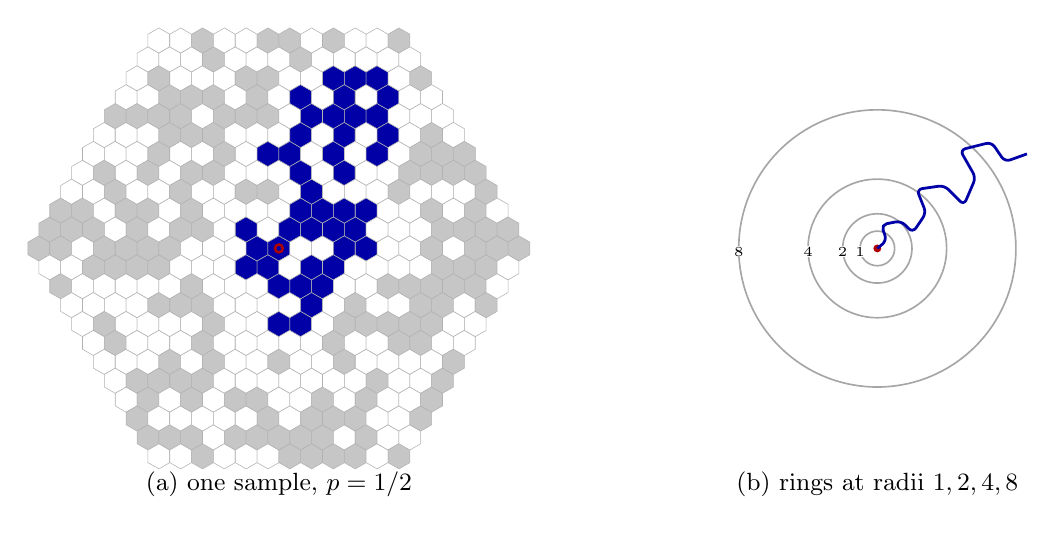
\begin{tikzpicture}
\begin{scope}
  \filldraw[fill=gray!45,draw=gray!60,line width=0.2pt] (-2.910,0.080) -- (-3.048,0.160) -- (-3.187,0.080) -- (-3.187,-0.080) -- (-3.048,-0.160) -- (-2.910,-0.080) -- cycle;
  \filldraw[fill=gray!45,draw=gray!60,line width=0.2pt] (-2.771,0.320) -- (-2.910,0.400) -- (-3.048,0.320) -- (-3.048,0.160) -- (-2.910,0.080) -- (-2.771,0.160) -- cycle;
  \filldraw[fill=gray!45,draw=gray!60,line width=0.2pt] (-2.633,0.560) -- (-2.771,0.640) -- (-2.910,0.560) -- (-2.910,0.400) -- (-2.771,0.320) -- (-2.633,0.400) -- cycle;
  \filldraw[fill=white,draw=gray!60,line width=0.2pt] (-2.494,0.800) -- (-2.633,0.880) -- (-2.771,0.800) -- (-2.771,0.640) -- (-2.633,0.560) -- (-2.494,0.640) -- cycle;
  \filldraw[fill=white,draw=gray!60,line width=0.2pt] (-2.356,1.040) -- (-2.494,1.120) -- (-2.633,1.040) -- (-2.633,0.880) -- (-2.494,0.800) -- (-2.356,0.880) -- cycle;
  \filldraw[fill=white,draw=gray!60,line width=0.2pt] (-2.217,1.280) -- (-2.356,1.360) -- (-2.494,1.280) -- (-2.494,1.120) -- (-2.356,1.040) -- (-2.217,1.120) -- cycle;
  \filldraw[fill=white,draw=gray!60,line width=0.2pt] (-2.078,1.520) -- (-2.217,1.600) -- (-2.356,1.520) -- (-2.356,1.360) -- (-2.217,1.280) -- (-2.078,1.360) -- cycle;
  \filldraw[fill=gray!45,draw=gray!60,line width=0.2pt] (-1.940,1.760) -- (-2.078,1.840) -- (-2.217,1.760) -- (-2.217,1.600) -- (-2.078,1.520) -- (-1.940,1.600) -- cycle;
  \filldraw[fill=white,draw=gray!60,line width=0.2pt] (-1.801,2.000) -- (-1.940,2.080) -- (-2.078,2.000) -- (-2.078,1.840) -- (-1.940,1.760) -- (-1.801,1.840) -- cycle;
  \filldraw[fill=white,draw=gray!60,line width=0.2pt] (-1.663,2.240) -- (-1.801,2.320) -- (-1.940,2.240) -- (-1.940,2.080) -- (-1.801,2.000) -- (-1.663,2.080) -- cycle;
  \filldraw[fill=white,draw=gray!60,line width=0.2pt] (-1.524,2.480) -- (-1.663,2.560) -- (-1.801,2.480) -- (-1.801,2.320) -- (-1.663,2.240) -- (-1.524,2.320) -- cycle;
  \filldraw[fill=white,draw=gray!60,line width=0.2pt] (-1.386,2.720) -- (-1.524,2.800) -- (-1.663,2.720) -- (-1.663,2.560) -- (-1.524,2.480) -- (-1.386,2.560) -- cycle;
  \filldraw[fill=white,draw=gray!60,line width=0.2pt] (-2.771,-0.160) -- (-2.910,-0.080) -- (-3.048,-0.160) -- (-3.048,-0.320) -- (-2.910,-0.400) -- (-2.771,-0.320) -- cycle;
  \filldraw[fill=gray!45,draw=gray!60,line width=0.2pt] (-2.633,0.080) -- (-2.771,0.160) -- (-2.910,0.080) -- (-2.910,-0.080) -- (-2.771,-0.160) -- (-2.633,-0.080) -- cycle;
  \filldraw[fill=gray!45,draw=gray!60,line width=0.2pt] (-2.494,0.320) -- (-2.633,0.400) -- (-2.771,0.320) -- (-2.771,0.160) -- (-2.633,0.080) -- (-2.494,0.160) -- cycle;
  \filldraw[fill=gray!45,draw=gray!60,line width=0.2pt] (-2.356,0.560) -- (-2.494,0.640) -- (-2.633,0.560) -- (-2.633,0.400) -- (-2.494,0.320) -- (-2.356,0.400) -- cycle;
  \filldraw[fill=white,draw=gray!60,line width=0.2pt] (-2.217,0.800) -- (-2.356,0.880) -- (-2.494,0.800) -- (-2.494,0.640) -- (-2.356,0.560) -- (-2.217,0.640) -- cycle;
  \filldraw[fill=gray!45,draw=gray!60,line width=0.2pt] (-2.078,1.040) -- (-2.217,1.120) -- (-2.356,1.040) -- (-2.356,0.880) -- (-2.217,0.800) -- (-2.078,0.880) -- cycle;
  \filldraw[fill=white,draw=gray!60,line width=0.2pt] (-1.940,1.280) -- (-2.078,1.360) -- (-2.217,1.280) -- (-2.217,1.120) -- (-2.078,1.040) -- (-1.940,1.120) -- cycle;
  \filldraw[fill=white,draw=gray!60,line width=0.2pt] (-1.801,1.520) -- (-1.940,1.600) -- (-2.078,1.520) -- (-2.078,1.360) -- (-1.940,1.280) -- (-1.801,1.360) -- cycle;
  \filldraw[fill=gray!45,draw=gray!60,line width=0.2pt] (-1.663,1.760) -- (-1.801,1.840) -- (-1.940,1.760) -- (-1.940,1.600) -- (-1.801,1.520) -- (-1.663,1.600) -- cycle;
  \filldraw[fill=white,draw=gray!60,line width=0.2pt] (-1.524,2.000) -- (-1.663,2.080) -- (-1.801,2.000) -- (-1.801,1.840) -- (-1.663,1.760) -- (-1.524,1.840) -- cycle;
  \filldraw[fill=gray!45,draw=gray!60,line width=0.2pt] (-1.386,2.240) -- (-1.524,2.320) -- (-1.663,2.240) -- (-1.663,2.080) -- (-1.524,2.000) -- (-1.386,2.080) -- cycle;
  \filldraw[fill=white,draw=gray!60,line width=0.2pt] (-1.247,2.480) -- (-1.386,2.560) -- (-1.524,2.480) -- (-1.524,2.320) -- (-1.386,2.240) -- (-1.247,2.320) -- cycle;
  \filldraw[fill=white,draw=gray!60,line width=0.2pt] (-1.109,2.720) -- (-1.247,2.800) -- (-1.386,2.720) -- (-1.386,2.560) -- (-1.247,2.480) -- (-1.109,2.560) -- cycle;
  \filldraw[fill=gray!45,draw=gray!60,line width=0.2pt] (-2.633,-0.400) -- (-2.771,-0.320) -- (-2.910,-0.400) -- (-2.910,-0.560) -- (-2.771,-0.640) -- (-2.633,-0.560) -- cycle;
  \filldraw[fill=white,draw=gray!60,line width=0.2pt] (-2.494,-0.160) -- (-2.633,-0.080) -- (-2.771,-0.160) -- (-2.771,-0.320) -- (-2.633,-0.400) -- (-2.494,-0.320) -- cycle;
  \filldraw[fill=white,draw=gray!60,line width=0.2pt] (-2.356,0.080) -- (-2.494,0.160) -- (-2.633,0.080) -- (-2.633,-0.080) -- (-2.494,-0.160) -- (-2.356,-0.080) -- cycle;
  \filldraw[fill=gray!45,draw=gray!60,line width=0.2pt] (-2.217,0.320) -- (-2.356,0.400) -- (-2.494,0.320) -- (-2.494,0.160) -- (-2.356,0.080) -- (-2.217,0.160) -- cycle;
  \filldraw[fill=white,draw=gray!60,line width=0.2pt] (-2.078,0.560) -- (-2.217,0.640) -- (-2.356,0.560) -- (-2.356,0.400) -- (-2.217,0.320) -- (-2.078,0.400) -- cycle;
  \filldraw[fill=gray!45,draw=gray!60,line width=0.2pt] (-1.940,0.800) -- (-2.078,0.880) -- (-2.217,0.800) -- (-2.217,0.640) -- (-2.078,0.560) -- (-1.940,0.640) -- cycle;
  \filldraw[fill=white,draw=gray!60,line width=0.2pt] (-1.801,1.040) -- (-1.940,1.120) -- (-2.078,1.040) -- (-2.078,0.880) -- (-1.940,0.800) -- (-1.801,0.880) -- cycle;
  \filldraw[fill=white,draw=gray!60,line width=0.2pt] (-1.663,1.280) -- (-1.801,1.360) -- (-1.940,1.280) -- (-1.940,1.120) -- (-1.801,1.040) -- (-1.663,1.120) -- cycle;
  \filldraw[fill=white,draw=gray!60,line width=0.2pt] (-1.524,1.520) -- (-1.663,1.600) -- (-1.801,1.520) -- (-1.801,1.360) -- (-1.663,1.280) -- (-1.524,1.360) -- cycle;
  \filldraw[fill=gray!45,draw=gray!60,line width=0.2pt] (-1.386,1.760) -- (-1.524,1.840) -- (-1.663,1.760) -- (-1.663,1.600) -- (-1.524,1.520) -- (-1.386,1.600) -- cycle;
  \filldraw[fill=gray!45,draw=gray!60,line width=0.2pt] (-1.247,2.000) -- (-1.386,2.080) -- (-1.524,2.000) -- (-1.524,1.840) -- (-1.386,1.760) -- (-1.247,1.840) -- cycle;
  \filldraw[fill=white,draw=gray!60,line width=0.2pt] (-1.109,2.240) -- (-1.247,2.320) -- (-1.386,2.240) -- (-1.386,2.080) -- (-1.247,2.000) -- (-1.109,2.080) -- cycle;
  \filldraw[fill=white,draw=gray!60,line width=0.2pt] (-0.970,2.480) -- (-1.109,2.560) -- (-1.247,2.480) -- (-1.247,2.320) -- (-1.109,2.240) -- (-0.970,2.320) -- cycle;
  \filldraw[fill=gray!45,draw=gray!60,line width=0.2pt] (-0.831,2.720) -- (-0.970,2.800) -- (-1.109,2.720) -- (-1.109,2.560) -- (-0.970,2.480) -- (-0.831,2.560) -- cycle;
  \filldraw[fill=white,draw=gray!60,line width=0.2pt] (-2.494,-0.640) -- (-2.633,-0.560) -- (-2.771,-0.640) -- (-2.771,-0.800) -- (-2.633,-0.880) -- (-2.494,-0.800) -- cycle;
  \filldraw[fill=white,draw=gray!60,line width=0.2pt] (-2.356,-0.400) -- (-2.494,-0.320) -- (-2.633,-0.400) -- (-2.633,-0.560) -- (-2.494,-0.640) -- (-2.356,-0.560) -- cycle;
  \filldraw[fill=gray!45,draw=gray!60,line width=0.2pt] (-2.217,-0.160) -- (-2.356,-0.080) -- (-2.494,-0.160) -- (-2.494,-0.320) -- (-2.356,-0.400) -- (-2.217,-0.320) -- cycle;
  \filldraw[fill=gray!45,draw=gray!60,line width=0.2pt] (-2.078,0.080) -- (-2.217,0.160) -- (-2.356,0.080) -- (-2.356,-0.080) -- (-2.217,-0.160) -- (-2.078,-0.080) -- cycle;
  \filldraw[fill=white,draw=gray!60,line width=0.2pt] (-1.940,0.320) -- (-2.078,0.400) -- (-2.217,0.320) -- (-2.217,0.160) -- (-2.078,0.080) -- (-1.940,0.160) -- cycle;
  \filldraw[fill=gray!45,draw=gray!60,line width=0.2pt] (-1.801,0.560) -- (-1.940,0.640) -- (-2.078,0.560) -- (-2.078,0.400) -- (-1.940,0.320) -- (-1.801,0.400) -- cycle;
  \filldraw[fill=white,draw=gray!60,line width=0.2pt] (-1.663,0.800) -- (-1.801,0.880) -- (-1.940,0.800) -- (-1.940,0.640) -- (-1.801,0.560) -- (-1.663,0.640) -- cycle;
  \filldraw[fill=gray!45,draw=gray!60,line width=0.2pt] (-1.524,1.040) -- (-1.663,1.120) -- (-1.801,1.040) -- (-1.801,0.880) -- (-1.663,0.800) -- (-1.524,0.880) -- cycle;
  \filldraw[fill=gray!45,draw=gray!60,line width=0.2pt] (-1.386,1.280) -- (-1.524,1.360) -- (-1.663,1.280) -- (-1.663,1.120) -- (-1.524,1.040) -- (-1.386,1.120) -- cycle;
  \filldraw[fill=gray!45,draw=gray!60,line width=0.2pt] (-1.247,1.520) -- (-1.386,1.600) -- (-1.524,1.520) -- (-1.524,1.360) -- (-1.386,1.280) -- (-1.247,1.360) -- cycle;
  \filldraw[fill=gray!45,draw=gray!60,line width=0.2pt] (-1.109,1.760) -- (-1.247,1.840) -- (-1.386,1.760) -- (-1.386,1.600) -- (-1.247,1.520) -- (-1.109,1.600) -- cycle;
  \filldraw[fill=gray!45,draw=gray!60,line width=0.2pt] (-0.970,2.000) -- (-1.109,2.080) -- (-1.247,2.000) -- (-1.247,1.840) -- (-1.109,1.760) -- (-0.970,1.840) -- cycle;
  \filldraw[fill=white,draw=gray!60,line width=0.2pt] (-0.831,2.240) -- (-0.970,2.320) -- (-1.109,2.240) -- (-1.109,2.080) -- (-0.970,2.000) -- (-0.831,2.080) -- cycle;
  \filldraw[fill=gray!45,draw=gray!60,line width=0.2pt] (-0.693,2.480) -- (-0.831,2.560) -- (-0.970,2.480) -- (-0.970,2.320) -- (-0.831,2.240) -- (-0.693,2.320) -- cycle;
  \filldraw[fill=white,draw=gray!60,line width=0.2pt] (-0.554,2.720) -- (-0.693,2.800) -- (-0.831,2.720) -- (-0.831,2.560) -- (-0.693,2.480) -- (-0.554,2.560) -- cycle;
  \filldraw[fill=white,draw=gray!60,line width=0.2pt] (-2.356,-0.880) -- (-2.494,-0.800) -- (-2.633,-0.880) -- (-2.633,-1.040) -- (-2.494,-1.120) -- (-2.356,-1.040) -- cycle;
  \filldraw[fill=white,draw=gray!60,line width=0.2pt] (-2.217,-0.640) -- (-2.356,-0.560) -- (-2.494,-0.640) -- (-2.494,-0.800) -- (-2.356,-0.880) -- (-2.217,-0.800) -- cycle;
  \filldraw[fill=white,draw=gray!60,line width=0.2pt] (-2.078,-0.400) -- (-2.217,-0.320) -- (-2.356,-0.400) -- (-2.356,-0.560) -- (-2.217,-0.640) -- (-2.078,-0.560) -- cycle;
  \filldraw[fill=gray!45,draw=gray!60,line width=0.2pt] (-1.940,-0.160) -- (-2.078,-0.080) -- (-2.217,-0.160) -- (-2.217,-0.320) -- (-2.078,-0.400) -- (-1.940,-0.320) -- cycle;
  \filldraw[fill=gray!45,draw=gray!60,line width=0.2pt] (-1.801,0.080) -- (-1.940,0.160) -- (-2.078,0.080) -- (-2.078,-0.080) -- (-1.940,-0.160) -- (-1.801,-0.080) -- cycle;
  \filldraw[fill=gray!45,draw=gray!60,line width=0.2pt] (-1.663,0.320) -- (-1.801,0.400) -- (-1.940,0.320) -- (-1.940,0.160) -- (-1.801,0.080) -- (-1.663,0.160) -- cycle;
  \filldraw[fill=gray!45,draw=gray!60,line width=0.2pt] (-1.524,0.560) -- (-1.663,0.640) -- (-1.801,0.560) -- (-1.801,0.400) -- (-1.663,0.320) -- (-1.524,0.400) -- cycle;
  \filldraw[fill=white,draw=gray!60,line width=0.2pt] (-1.386,0.800) -- (-1.524,0.880) -- (-1.663,0.800) -- (-1.663,0.640) -- (-1.524,0.560) -- (-1.386,0.640) -- cycle;
  \filldraw[fill=white,draw=gray!60,line width=0.2pt] (-1.247,1.040) -- (-1.386,1.120) -- (-1.524,1.040) -- (-1.524,0.880) -- (-1.386,0.800) -- (-1.247,0.880) -- cycle;
  \filldraw[fill=white,draw=gray!60,line width=0.2pt] (-1.109,1.280) -- (-1.247,1.360) -- (-1.386,1.280) -- (-1.386,1.120) -- (-1.247,1.040) -- (-1.109,1.120) -- cycle;
  \filldraw[fill=gray!45,draw=gray!60,line width=0.2pt] (-0.970,1.520) -- (-1.109,1.600) -- (-1.247,1.520) -- (-1.247,1.360) -- (-1.109,1.280) -- (-0.970,1.360) -- cycle;
  \filldraw[fill=white,draw=gray!60,line width=0.2pt] (-0.831,1.760) -- (-0.970,1.840) -- (-1.109,1.760) -- (-1.109,1.600) -- (-0.970,1.520) -- (-0.831,1.600) -- cycle;
  \filldraw[fill=gray!45,draw=gray!60,line width=0.2pt] (-0.693,2.000) -- (-0.831,2.080) -- (-0.970,2.000) -- (-0.970,1.840) -- (-0.831,1.760) -- (-0.693,1.840) -- cycle;
  \filldraw[fill=white,draw=gray!60,line width=0.2pt] (-0.554,2.240) -- (-0.693,2.320) -- (-0.831,2.240) -- (-0.831,2.080) -- (-0.693,2.000) -- (-0.554,2.080) -- cycle;
  \filldraw[fill=white,draw=gray!60,line width=0.2pt] (-0.416,2.480) -- (-0.554,2.560) -- (-0.693,2.480) -- (-0.693,2.320) -- (-0.554,2.240) -- (-0.416,2.320) -- cycle;
  \filldraw[fill=white,draw=gray!60,line width=0.2pt] (-0.277,2.720) -- (-0.416,2.800) -- (-0.554,2.720) -- (-0.554,2.560) -- (-0.416,2.480) -- (-0.277,2.560) -- cycle;
  \filldraw[fill=white,draw=gray!60,line width=0.2pt] (-2.217,-1.120) -- (-2.356,-1.040) -- (-2.494,-1.120) -- (-2.494,-1.280) -- (-2.356,-1.360) -- (-2.217,-1.280) -- cycle;
  \filldraw[fill=gray!45,draw=gray!60,line width=0.2pt] (-2.078,-0.880) -- (-2.217,-0.800) -- (-2.356,-0.880) -- (-2.356,-1.040) -- (-2.217,-1.120) -- (-2.078,-1.040) -- cycle;
  \filldraw[fill=white,draw=gray!60,line width=0.2pt] (-1.940,-0.640) -- (-2.078,-0.560) -- (-2.217,-0.640) -- (-2.217,-0.800) -- (-2.078,-0.880) -- (-1.940,-0.800) -- cycle;
  \filldraw[fill=white,draw=gray!60,line width=0.2pt] (-1.801,-0.400) -- (-1.940,-0.320) -- (-2.078,-0.400) -- (-2.078,-0.560) -- (-1.940,-0.640) -- (-1.801,-0.560) -- cycle;
  \filldraw[fill=gray!45,draw=gray!60,line width=0.2pt] (-1.663,-0.160) -- (-1.801,-0.080) -- (-1.940,-0.160) -- (-1.940,-0.320) -- (-1.801,-0.400) -- (-1.663,-0.320) -- cycle;
  \filldraw[fill=gray!45,draw=gray!60,line width=0.2pt] (-1.524,0.080) -- (-1.663,0.160) -- (-1.801,0.080) -- (-1.801,-0.080) -- (-1.663,-0.160) -- (-1.524,-0.080) -- cycle;
  \filldraw[fill=white,draw=gray!60,line width=0.2pt] (-1.386,0.320) -- (-1.524,0.400) -- (-1.663,0.320) -- (-1.663,0.160) -- (-1.524,0.080) -- (-1.386,0.160) -- cycle;
  \filldraw[fill=white,draw=gray!60,line width=0.2pt] (-1.247,0.560) -- (-1.386,0.640) -- (-1.524,0.560) -- (-1.524,0.400) -- (-1.386,0.320) -- (-1.247,0.400) -- cycle;
  \filldraw[fill=gray!45,draw=gray!60,line width=0.2pt] (-1.109,0.800) -- (-1.247,0.880) -- (-1.386,0.800) -- (-1.386,0.640) -- (-1.247,0.560) -- (-1.109,0.640) -- cycle;
  \filldraw[fill=gray!45,draw=gray!60,line width=0.2pt] (-0.970,1.040) -- (-1.109,1.120) -- (-1.247,1.040) -- (-1.247,0.880) -- (-1.109,0.800) -- (-0.970,0.880) -- cycle;
  \filldraw[fill=white,draw=gray!60,line width=0.2pt] (-0.831,1.280) -- (-0.970,1.360) -- (-1.109,1.280) -- (-1.109,1.120) -- (-0.970,1.040) -- (-0.831,1.120) -- cycle;
  \filldraw[fill=gray!45,draw=gray!60,line width=0.2pt] (-0.693,1.520) -- (-0.831,1.600) -- (-0.970,1.520) -- (-0.970,1.360) -- (-0.831,1.280) -- (-0.693,1.360) -- cycle;
  \filldraw[fill=gray!45,draw=gray!60,line width=0.2pt] (-0.554,1.760) -- (-0.693,1.840) -- (-0.831,1.760) -- (-0.831,1.600) -- (-0.693,1.520) -- (-0.554,1.600) -- cycle;
  \filldraw[fill=white,draw=gray!60,line width=0.2pt] (-0.416,2.000) -- (-0.554,2.080) -- (-0.693,2.000) -- (-0.693,1.840) -- (-0.554,1.760) -- (-0.416,1.840) -- cycle;
  \filldraw[fill=gray!45,draw=gray!60,line width=0.2pt] (-0.277,2.240) -- (-0.416,2.320) -- (-0.554,2.240) -- (-0.554,2.080) -- (-0.416,2.000) -- (-0.277,2.080) -- cycle;
  \filldraw[fill=white,draw=gray!60,line width=0.2pt] (-0.139,2.480) -- (-0.277,2.560) -- (-0.416,2.480) -- (-0.416,2.320) -- (-0.277,2.240) -- (-0.139,2.320) -- cycle;
  \filldraw[fill=gray!45,draw=gray!60,line width=0.2pt] (0.000,2.720) -- (-0.139,2.800) -- (-0.277,2.720) -- (-0.277,2.560) -- (-0.139,2.480) -- (-0.000,2.560) -- cycle;
  \filldraw[fill=white,draw=gray!60,line width=0.2pt] (-2.078,-1.360) -- (-2.217,-1.280) -- (-2.356,-1.360) -- (-2.356,-1.520) -- (-2.217,-1.600) -- (-2.078,-1.520) -- cycle;
  \filldraw[fill=gray!45,draw=gray!60,line width=0.2pt] (-1.940,-1.120) -- (-2.078,-1.040) -- (-2.217,-1.120) -- (-2.217,-1.280) -- (-2.078,-1.360) -- (-1.940,-1.280) -- cycle;
  \filldraw[fill=white,draw=gray!60,line width=0.2pt] (-1.801,-0.880) -- (-1.940,-0.800) -- (-2.078,-0.880) -- (-2.078,-1.040) -- (-1.940,-1.120) -- (-1.801,-1.040) -- cycle;
  \filldraw[fill=white,draw=gray!60,line width=0.2pt] (-1.663,-0.640) -- (-1.801,-0.560) -- (-1.940,-0.640) -- (-1.940,-0.800) -- (-1.801,-0.880) -- (-1.663,-0.800) -- cycle;
  \filldraw[fill=white,draw=gray!60,line width=0.2pt] (-1.524,-0.400) -- (-1.663,-0.320) -- (-1.801,-0.400) -- (-1.801,-0.560) -- (-1.663,-0.640) -- (-1.524,-0.560) -- cycle;
  \filldraw[fill=gray!45,draw=gray!60,line width=0.2pt] (-1.386,-0.160) -- (-1.524,-0.080) -- (-1.663,-0.160) -- (-1.663,-0.320) -- (-1.524,-0.400) -- (-1.386,-0.320) -- cycle;
  \filldraw[fill=gray!45,draw=gray!60,line width=0.2pt] (-1.247,0.080) -- (-1.386,0.160) -- (-1.524,0.080) -- (-1.524,-0.080) -- (-1.386,-0.160) -- (-1.247,-0.080) -- cycle;
  \filldraw[fill=gray!45,draw=gray!60,line width=0.2pt] (-1.109,0.320) -- (-1.247,0.400) -- (-1.386,0.320) -- (-1.386,0.160) -- (-1.247,0.080) -- (-1.109,0.160) -- cycle;
  \filldraw[fill=gray!45,draw=gray!60,line width=0.2pt] (-0.970,0.560) -- (-1.109,0.640) -- (-1.247,0.560) -- (-1.247,0.400) -- (-1.109,0.320) -- (-0.970,0.400) -- cycle;
  \filldraw[fill=white,draw=gray!60,line width=0.2pt] (-0.831,0.800) -- (-0.970,0.880) -- (-1.109,0.800) -- (-1.109,0.640) -- (-0.970,0.560) -- (-0.831,0.640) -- cycle;
  \filldraw[fill=gray!45,draw=gray!60,line width=0.2pt] (-0.693,1.040) -- (-0.831,1.120) -- (-0.970,1.040) -- (-0.970,0.880) -- (-0.831,0.800) -- (-0.693,0.880) -- cycle;
  \filldraw[fill=gray!45,draw=gray!60,line width=0.2pt] (-0.554,1.280) -- (-0.693,1.360) -- (-0.831,1.280) -- (-0.831,1.120) -- (-0.693,1.040) -- (-0.554,1.120) -- cycle;
  \filldraw[fill=white,draw=gray!60,line width=0.2pt] (-0.416,1.520) -- (-0.554,1.600) -- (-0.693,1.520) -- (-0.693,1.360) -- (-0.554,1.280) -- (-0.416,1.360) -- cycle;
  \filldraw[fill=gray!45,draw=gray!60,line width=0.2pt] (-0.277,1.760) -- (-0.416,1.840) -- (-0.554,1.760) -- (-0.554,1.600) -- (-0.416,1.520) -- (-0.277,1.600) -- cycle;
  \filldraw[fill=gray!45,draw=gray!60,line width=0.2pt] (-0.139,2.000) -- (-0.277,2.080) -- (-0.416,2.000) -- (-0.416,1.840) -- (-0.277,1.760) -- (-0.139,1.840) -- cycle;
  \filldraw[fill=gray!45,draw=gray!60,line width=0.2pt] (0.000,2.240) -- (-0.139,2.320) -- (-0.277,2.240) -- (-0.277,2.080) -- (-0.139,2.000) -- (-0.000,2.080) -- cycle;
  \filldraw[fill=white,draw=gray!60,line width=0.2pt] (0.139,2.480) -- (0.000,2.560) -- (-0.139,2.480) -- (-0.139,2.320) -- (-0.000,2.240) -- (0.139,2.320) -- cycle;
  \filldraw[fill=gray!45,draw=gray!60,line width=0.2pt] (0.277,2.720) -- (0.139,2.800) -- (0.000,2.720) -- (0.000,2.560) -- (0.139,2.480) -- (0.277,2.560) -- cycle;
  \filldraw[fill=white,draw=gray!60,line width=0.2pt] (-1.940,-1.600) -- (-2.078,-1.520) -- (-2.217,-1.600) -- (-2.217,-1.760) -- (-2.078,-1.840) -- (-1.940,-1.760) -- cycle;
  \filldraw[fill=white,draw=gray!60,line width=0.2pt] (-1.801,-1.360) -- (-1.940,-1.280) -- (-2.078,-1.360) -- (-2.078,-1.520) -- (-1.940,-1.600) -- (-1.801,-1.520) -- cycle;
  \filldraw[fill=white,draw=gray!60,line width=0.2pt] (-1.663,-1.120) -- (-1.801,-1.040) -- (-1.940,-1.120) -- (-1.940,-1.280) -- (-1.801,-1.360) -- (-1.663,-1.280) -- cycle;
  \filldraw[fill=white,draw=gray!60,line width=0.2pt] (-1.524,-0.880) -- (-1.663,-0.800) -- (-1.801,-0.880) -- (-1.801,-1.040) -- (-1.663,-1.120) -- (-1.524,-1.040) -- cycle;
  \filldraw[fill=gray!45,draw=gray!60,line width=0.2pt] (-1.386,-0.640) -- (-1.524,-0.560) -- (-1.663,-0.640) -- (-1.663,-0.800) -- (-1.524,-0.880) -- (-1.386,-0.800) -- cycle;
  \filldraw[fill=white,draw=gray!60,line width=0.2pt] (-1.247,-0.400) -- (-1.386,-0.320) -- (-1.524,-0.400) -- (-1.524,-0.560) -- (-1.386,-0.640) -- (-1.247,-0.560) -- cycle;
  \filldraw[fill=white,draw=gray!60,line width=0.2pt] (-1.109,-0.160) -- (-1.247,-0.080) -- (-1.386,-0.160) -- (-1.386,-0.320) -- (-1.247,-0.400) -- (-1.109,-0.320) -- cycle;
  \filldraw[fill=white,draw=gray!60,line width=0.2pt] (-0.970,0.080) -- (-1.109,0.160) -- (-1.247,0.080) -- (-1.247,-0.080) -- (-1.109,-0.160) -- (-0.970,-0.080) -- cycle;
  \filldraw[fill=gray!45,draw=gray!60,line width=0.2pt] (-0.831,0.320) -- (-0.970,0.400) -- (-1.109,0.320) -- (-1.109,0.160) -- (-0.970,0.080) -- (-0.831,0.160) -- cycle;
  \filldraw[fill=white,draw=gray!60,line width=0.2pt] (-0.693,0.560) -- (-0.831,0.640) -- (-0.970,0.560) -- (-0.970,0.400) -- (-0.831,0.320) -- (-0.693,0.400) -- cycle;
  \filldraw[fill=white,draw=gray!60,line width=0.2pt] (-0.554,0.800) -- (-0.693,0.880) -- (-0.831,0.800) -- (-0.831,0.640) -- (-0.693,0.560) -- (-0.554,0.640) -- cycle;
  \filldraw[fill=white,draw=gray!60,line width=0.2pt] (-0.416,1.040) -- (-0.554,1.120) -- (-0.693,1.040) -- (-0.693,0.880) -- (-0.554,0.800) -- (-0.416,0.880) -- cycle;
  \filldraw[fill=white,draw=gray!60,line width=0.2pt] (-0.277,1.280) -- (-0.416,1.360) -- (-0.554,1.280) -- (-0.554,1.120) -- (-0.416,1.040) -- (-0.277,1.120) -- cycle;
  \filldraw[fill=white,draw=gray!60,line width=0.2pt] (-0.139,1.520) -- (-0.277,1.600) -- (-0.416,1.520) -- (-0.416,1.360) -- (-0.277,1.280) -- (-0.139,1.360) -- cycle;
  \filldraw[fill=gray!45,draw=gray!60,line width=0.2pt] (0.000,1.760) -- (-0.139,1.840) -- (-0.277,1.760) -- (-0.277,1.600) -- (-0.139,1.520) -- (-0.000,1.600) -- cycle;
  \filldraw[fill=white,draw=gray!60,line width=0.2pt] (0.139,2.000) -- (0.000,2.080) -- (-0.139,2.000) -- (-0.139,1.840) -- (-0.000,1.760) -- (0.139,1.840) -- cycle;
  \filldraw[fill=white,draw=gray!60,line width=0.2pt] (0.277,2.240) -- (0.139,2.320) -- (0.000,2.240) -- (0.000,2.080) -- (0.139,2.000) -- (0.277,2.080) -- cycle;
  \filldraw[fill=gray!45,draw=gray!60,line width=0.2pt] (0.416,2.480) -- (0.277,2.560) -- (0.139,2.480) -- (0.139,2.320) -- (0.277,2.240) -- (0.416,2.320) -- cycle;
  \filldraw[fill=white,draw=gray!60,line width=0.2pt] (0.554,2.720) -- (0.416,2.800) -- (0.277,2.720) -- (0.277,2.560) -- (0.416,2.480) -- (0.554,2.560) -- cycle;
  \filldraw[fill=white,draw=gray!60,line width=0.2pt] (-1.801,-1.840) -- (-1.940,-1.760) -- (-2.078,-1.840) -- (-2.078,-2.000) -- (-1.940,-2.080) -- (-1.801,-2.000) -- cycle;
  \filldraw[fill=gray!45,draw=gray!60,line width=0.2pt] (-1.663,-1.600) -- (-1.801,-1.520) -- (-1.940,-1.600) -- (-1.940,-1.760) -- (-1.801,-1.840) -- (-1.663,-1.760) -- cycle;
  \filldraw[fill=white,draw=gray!60,line width=0.2pt] (-1.524,-1.360) -- (-1.663,-1.280) -- (-1.801,-1.360) -- (-1.801,-1.520) -- (-1.663,-1.600) -- (-1.524,-1.520) -- cycle;
  \filldraw[fill=white,draw=gray!60,line width=0.2pt] (-1.386,-1.120) -- (-1.524,-1.040) -- (-1.663,-1.120) -- (-1.663,-1.280) -- (-1.524,-1.360) -- (-1.386,-1.280) -- cycle;
  \filldraw[fill=white,draw=gray!60,line width=0.2pt] (-1.247,-0.880) -- (-1.386,-0.800) -- (-1.524,-0.880) -- (-1.524,-1.040) -- (-1.386,-1.120) -- (-1.247,-1.040) -- cycle;
  \filldraw[fill=gray!45,draw=gray!60,line width=0.2pt] (-1.109,-0.640) -- (-1.247,-0.560) -- (-1.386,-0.640) -- (-1.386,-0.800) -- (-1.247,-0.880) -- (-1.109,-0.800) -- cycle;
  \filldraw[fill=gray!45,draw=gray!60,line width=0.2pt] (-0.970,-0.400) -- (-1.109,-0.320) -- (-1.247,-0.400) -- (-1.247,-0.560) -- (-1.109,-0.640) -- (-0.970,-0.560) -- cycle;
  \filldraw[fill=white,draw=gray!60,line width=0.2pt] (-0.831,-0.160) -- (-0.970,-0.080) -- (-1.109,-0.160) -- (-1.109,-0.320) -- (-0.970,-0.400) -- (-0.831,-0.320) -- cycle;
  \filldraw[fill=white,draw=gray!60,line width=0.2pt] (-0.693,0.080) -- (-0.831,0.160) -- (-0.970,0.080) -- (-0.970,-0.080) -- (-0.831,-0.160) -- (-0.693,-0.080) -- cycle;
  \filldraw[fill=white,draw=gray!60,line width=0.2pt] (-0.554,0.320) -- (-0.693,0.400) -- (-0.831,0.320) -- (-0.831,0.160) -- (-0.693,0.080) -- (-0.554,0.160) -- cycle;
  \filldraw[fill=white,draw=gray!60,line width=0.2pt] (-0.416,0.560) -- (-0.554,0.640) -- (-0.693,0.560) -- (-0.693,0.400) -- (-0.554,0.320) -- (-0.416,0.400) -- cycle;
  \filldraw[fill=gray!45,draw=gray!60,line width=0.2pt] (-0.277,0.800) -- (-0.416,0.880) -- (-0.554,0.800) -- (-0.554,0.640) -- (-0.416,0.560) -- (-0.277,0.640) -- cycle;
  \filldraw[fill=white,draw=gray!60,line width=0.2pt] (-0.139,1.040) -- (-0.277,1.120) -- (-0.416,1.040) -- (-0.416,0.880) -- (-0.277,0.800) -- (-0.139,0.880) -- cycle;
  \filldraw[fill=blue!65!black,draw=gray!60,line width=0.2pt] (0.000,1.280) -- (-0.139,1.360) -- (-0.277,1.280) -- (-0.277,1.120) -- (-0.139,1.040) -- (-0.000,1.120) -- cycle;
  \filldraw[fill=white,draw=gray!60,line width=0.2pt] (0.139,1.520) -- (0.000,1.600) -- (-0.139,1.520) -- (-0.139,1.360) -- (-0.000,1.280) -- (0.139,1.360) -- cycle;
  \filldraw[fill=white,draw=gray!60,line width=0.2pt] (0.277,1.760) -- (0.139,1.840) -- (0.000,1.760) -- (0.000,1.600) -- (0.139,1.520) -- (0.277,1.600) -- cycle;
  \filldraw[fill=blue!65!black,draw=gray!60,line width=0.2pt] (0.416,2.000) -- (0.277,2.080) -- (0.139,2.000) -- (0.139,1.840) -- (0.277,1.760) -- (0.416,1.840) -- cycle;
  \filldraw[fill=white,draw=gray!60,line width=0.2pt] (0.554,2.240) -- (0.416,2.320) -- (0.277,2.240) -- (0.277,2.080) -- (0.416,2.000) -- (0.554,2.080) -- cycle;
  \filldraw[fill=white,draw=gray!60,line width=0.2pt] (0.693,2.480) -- (0.554,2.560) -- (0.416,2.480) -- (0.416,2.320) -- (0.554,2.240) -- (0.693,2.320) -- cycle;
  \filldraw[fill=gray!45,draw=gray!60,line width=0.2pt] (0.831,2.720) -- (0.693,2.800) -- (0.554,2.720) -- (0.554,2.560) -- (0.693,2.480) -- (0.831,2.560) -- cycle;
  \filldraw[fill=gray!45,draw=gray!60,line width=0.2pt] (-1.663,-2.080) -- (-1.801,-2.000) -- (-1.940,-2.080) -- (-1.940,-2.240) -- (-1.801,-2.320) -- (-1.663,-2.240) -- cycle;
  \filldraw[fill=gray!45,draw=gray!60,line width=0.2pt] (-1.524,-1.840) -- (-1.663,-1.760) -- (-1.801,-1.840) -- (-1.801,-2.000) -- (-1.663,-2.080) -- (-1.524,-2.000) -- cycle;
  \filldraw[fill=gray!45,draw=gray!60,line width=0.2pt] (-1.386,-1.600) -- (-1.524,-1.520) -- (-1.663,-1.600) -- (-1.663,-1.760) -- (-1.524,-1.840) -- (-1.386,-1.760) -- cycle;
  \filldraw[fill=gray!45,draw=gray!60,line width=0.2pt] (-1.247,-1.360) -- (-1.386,-1.280) -- (-1.524,-1.360) -- (-1.524,-1.520) -- (-1.386,-1.600) -- (-1.247,-1.520) -- cycle;
  \filldraw[fill=white,draw=gray!60,line width=0.2pt] (-1.109,-1.120) -- (-1.247,-1.040) -- (-1.386,-1.120) -- (-1.386,-1.280) -- (-1.247,-1.360) -- (-1.109,-1.280) -- cycle;
  \filldraw[fill=white,draw=gray!60,line width=0.2pt] (-0.970,-0.880) -- (-1.109,-0.800) -- (-1.247,-0.880) -- (-1.247,-1.040) -- (-1.109,-1.120) -- (-0.970,-1.040) -- cycle;
  \filldraw[fill=gray!45,draw=gray!60,line width=0.2pt] (-0.831,-0.640) -- (-0.970,-0.560) -- (-1.109,-0.640) -- (-1.109,-0.800) -- (-0.970,-0.880) -- (-0.831,-0.800) -- cycle;
  \filldraw[fill=white,draw=gray!60,line width=0.2pt] (-0.693,-0.400) -- (-0.831,-0.320) -- (-0.970,-0.400) -- (-0.970,-0.560) -- (-0.831,-0.640) -- (-0.693,-0.560) -- cycle;
  \filldraw[fill=white,draw=gray!60,line width=0.2pt] (-0.554,-0.160) -- (-0.693,-0.080) -- (-0.831,-0.160) -- (-0.831,-0.320) -- (-0.693,-0.400) -- (-0.554,-0.320) -- cycle;
  \filldraw[fill=white,draw=gray!60,line width=0.2pt] (-0.416,0.080) -- (-0.554,0.160) -- (-0.693,0.080) -- (-0.693,-0.080) -- (-0.554,-0.160) -- (-0.416,-0.080) -- cycle;
  \filldraw[fill=blue!65!black,draw=gray!60,line width=0.2pt] (-0.277,0.320) -- (-0.416,0.400) -- (-0.554,0.320) -- (-0.554,0.160) -- (-0.416,0.080) -- (-0.277,0.160) -- cycle;
  \filldraw[fill=white,draw=gray!60,line width=0.2pt] (-0.139,0.560) -- (-0.277,0.640) -- (-0.416,0.560) -- (-0.416,0.400) -- (-0.277,0.320) -- (-0.139,0.400) -- cycle;
  \filldraw[fill=gray!45,draw=gray!60,line width=0.2pt] (0.000,0.800) -- (-0.139,0.880) -- (-0.277,0.800) -- (-0.277,0.640) -- (-0.139,0.560) -- (-0.000,0.640) -- cycle;
  \filldraw[fill=white,draw=gray!60,line width=0.2pt] (0.139,1.040) -- (0.000,1.120) -- (-0.139,1.040) -- (-0.139,0.880) -- (-0.000,0.800) -- (0.139,0.880) -- cycle;
  \filldraw[fill=blue!65!black,draw=gray!60,line width=0.2pt] (0.277,1.280) -- (0.139,1.360) -- (0.000,1.280) -- (0.000,1.120) -- (0.139,1.040) -- (0.277,1.120) -- cycle;
  \filldraw[fill=blue!65!black,draw=gray!60,line width=0.2pt] (0.416,1.520) -- (0.277,1.600) -- (0.139,1.520) -- (0.139,1.360) -- (0.277,1.280) -- (0.416,1.360) -- cycle;
  \filldraw[fill=blue!65!black,draw=gray!60,line width=0.2pt] (0.554,1.760) -- (0.416,1.840) -- (0.277,1.760) -- (0.277,1.600) -- (0.416,1.520) -- (0.554,1.600) -- cycle;
  \filldraw[fill=white,draw=gray!60,line width=0.2pt] (0.693,2.000) -- (0.554,2.080) -- (0.416,2.000) -- (0.416,1.840) -- (0.554,1.760) -- (0.693,1.840) -- cycle;
  \filldraw[fill=blue!65!black,draw=gray!60,line width=0.2pt] (0.831,2.240) -- (0.693,2.320) -- (0.554,2.240) -- (0.554,2.080) -- (0.693,2.000) -- (0.831,2.080) -- cycle;
  \filldraw[fill=white,draw=gray!60,line width=0.2pt] (0.970,2.480) -- (0.831,2.560) -- (0.693,2.480) -- (0.693,2.320) -- (0.831,2.240) -- (0.970,2.320) -- cycle;
  \filldraw[fill=white,draw=gray!60,line width=0.2pt] (1.109,2.720) -- (0.970,2.800) -- (0.831,2.720) -- (0.831,2.560) -- (0.970,2.480) -- (1.109,2.560) -- cycle;
  \filldraw[fill=gray!45,draw=gray!60,line width=0.2pt] (-1.524,-2.320) -- (-1.663,-2.240) -- (-1.801,-2.320) -- (-1.801,-2.480) -- (-1.663,-2.560) -- (-1.524,-2.480) -- cycle;
  \filldraw[fill=white,draw=gray!60,line width=0.2pt] (-1.386,-2.080) -- (-1.524,-2.000) -- (-1.663,-2.080) -- (-1.663,-2.240) -- (-1.524,-2.320) -- (-1.386,-2.240) -- cycle;
  \filldraw[fill=white,draw=gray!60,line width=0.2pt] (-1.247,-1.840) -- (-1.386,-1.760) -- (-1.524,-1.840) -- (-1.524,-2.000) -- (-1.386,-2.080) -- (-1.247,-2.000) -- cycle;
  \filldraw[fill=gray!45,draw=gray!60,line width=0.2pt] (-1.109,-1.600) -- (-1.247,-1.520) -- (-1.386,-1.600) -- (-1.386,-1.760) -- (-1.247,-1.840) -- (-1.109,-1.760) -- cycle;
  \filldraw[fill=white,draw=gray!60,line width=0.2pt] (-0.970,-1.360) -- (-1.109,-1.280) -- (-1.247,-1.360) -- (-1.247,-1.520) -- (-1.109,-1.600) -- (-0.970,-1.520) -- cycle;
  \filldraw[fill=gray!45,draw=gray!60,line width=0.2pt] (-0.831,-1.120) -- (-0.970,-1.040) -- (-1.109,-1.120) -- (-1.109,-1.280) -- (-0.970,-1.360) -- (-0.831,-1.280) -- cycle;
  \filldraw[fill=gray!45,draw=gray!60,line width=0.2pt] (-0.693,-0.880) -- (-0.831,-0.800) -- (-0.970,-0.880) -- (-0.970,-1.040) -- (-0.831,-1.120) -- (-0.693,-1.040) -- cycle;
  \filldraw[fill=white,draw=gray!60,line width=0.2pt] (-0.554,-0.640) -- (-0.693,-0.560) -- (-0.831,-0.640) -- (-0.831,-0.800) -- (-0.693,-0.880) -- (-0.554,-0.800) -- cycle;
  \filldraw[fill=white,draw=gray!60,line width=0.2pt] (-0.416,-0.400) -- (-0.554,-0.320) -- (-0.693,-0.400) -- (-0.693,-0.560) -- (-0.554,-0.640) -- (-0.416,-0.560) -- cycle;
  \filldraw[fill=blue!65!black,draw=gray!60,line width=0.2pt] (-0.277,-0.160) -- (-0.416,-0.080) -- (-0.554,-0.160) -- (-0.554,-0.320) -- (-0.416,-0.400) -- (-0.277,-0.320) -- cycle;
  \filldraw[fill=blue!65!black,draw=gray!60,line width=0.2pt] (-0.139,0.080) -- (-0.277,0.160) -- (-0.416,0.080) -- (-0.416,-0.080) -- (-0.277,-0.160) -- (-0.139,-0.080) -- cycle;
  \filldraw[fill=white,draw=gray!60,line width=0.2pt] (0.000,0.320) -- (-0.139,0.400) -- (-0.277,0.320) -- (-0.277,0.160) -- (-0.139,0.080) -- (-0.000,0.160) -- cycle;
  \filldraw[fill=white,draw=gray!60,line width=0.2pt] (0.139,0.560) -- (0.000,0.640) -- (-0.139,0.560) -- (-0.139,0.400) -- (-0.000,0.320) -- (0.139,0.400) -- cycle;
  \filldraw[fill=white,draw=gray!60,line width=0.2pt] (0.277,0.800) -- (0.139,0.880) -- (0.000,0.800) -- (0.000,0.640) -- (0.139,0.560) -- (0.277,0.640) -- cycle;
  \filldraw[fill=blue!65!black,draw=gray!60,line width=0.2pt] (0.416,1.040) -- (0.277,1.120) -- (0.139,1.040) -- (0.139,0.880) -- (0.277,0.800) -- (0.416,0.880) -- cycle;
  \filldraw[fill=white,draw=gray!60,line width=0.2pt] (0.554,1.280) -- (0.416,1.360) -- (0.277,1.280) -- (0.277,1.120) -- (0.416,1.040) -- (0.554,1.120) -- cycle;
  \filldraw[fill=white,draw=gray!60,line width=0.2pt] (0.693,1.520) -- (0.554,1.600) -- (0.416,1.520) -- (0.416,1.360) -- (0.554,1.280) -- (0.693,1.360) -- cycle;
  \filldraw[fill=blue!65!black,draw=gray!60,line width=0.2pt] (0.831,1.760) -- (0.693,1.840) -- (0.554,1.760) -- (0.554,1.600) -- (0.693,1.520) -- (0.831,1.600) -- cycle;
  \filldraw[fill=blue!65!black,draw=gray!60,line width=0.2pt] (0.970,2.000) -- (0.831,2.080) -- (0.693,2.000) -- (0.693,1.840) -- (0.831,1.760) -- (0.970,1.840) -- cycle;
  \filldraw[fill=blue!65!black,draw=gray!60,line width=0.2pt] (1.109,2.240) -- (0.970,2.320) -- (0.831,2.240) -- (0.831,2.080) -- (0.970,2.000) -- (1.109,2.080) -- cycle;
  \filldraw[fill=white,draw=gray!60,line width=0.2pt] (1.247,2.480) -- (1.109,2.560) -- (0.970,2.480) -- (0.970,2.320) -- (1.109,2.240) -- (1.247,2.320) -- cycle;
  \filldraw[fill=white,draw=gray!60,line width=0.2pt] (1.386,2.720) -- (1.247,2.800) -- (1.109,2.720) -- (1.109,2.560) -- (1.247,2.480) -- (1.386,2.560) -- cycle;
  \filldraw[fill=white,draw=gray!60,line width=0.2pt] (-1.386,-2.560) -- (-1.524,-2.480) -- (-1.663,-2.560) -- (-1.663,-2.720) -- (-1.524,-2.800) -- (-1.386,-2.720) -- cycle;
  \filldraw[fill=gray!45,draw=gray!60,line width=0.2pt] (-1.247,-2.320) -- (-1.386,-2.240) -- (-1.524,-2.320) -- (-1.524,-2.480) -- (-1.386,-2.560) -- (-1.247,-2.480) -- cycle;
  \filldraw[fill=white,draw=gray!60,line width=0.2pt] (-1.109,-2.080) -- (-1.247,-2.000) -- (-1.386,-2.080) -- (-1.386,-2.240) -- (-1.247,-2.320) -- (-1.109,-2.240) -- cycle;
  \filldraw[fill=gray!45,draw=gray!60,line width=0.2pt] (-0.970,-1.840) -- (-1.109,-1.760) -- (-1.247,-1.840) -- (-1.247,-2.000) -- (-1.109,-2.080) -- (-0.970,-2.000) -- cycle;
  \filldraw[fill=gray!45,draw=gray!60,line width=0.2pt] (-0.831,-1.600) -- (-0.970,-1.520) -- (-1.109,-1.600) -- (-1.109,-1.760) -- (-0.970,-1.840) -- (-0.831,-1.760) -- cycle;
  \filldraw[fill=gray!45,draw=gray!60,line width=0.2pt] (-0.693,-1.360) -- (-0.831,-1.280) -- (-0.970,-1.360) -- (-0.970,-1.520) -- (-0.831,-1.600) -- (-0.693,-1.520) -- cycle;
  \filldraw[fill=white,draw=gray!60,line width=0.2pt] (-0.554,-1.120) -- (-0.693,-1.040) -- (-0.831,-1.120) -- (-0.831,-1.280) -- (-0.693,-1.360) -- (-0.554,-1.280) -- cycle;
  \filldraw[fill=white,draw=gray!60,line width=0.2pt] (-0.416,-0.880) -- (-0.554,-0.800) -- (-0.693,-0.880) -- (-0.693,-1.040) -- (-0.554,-1.120) -- (-0.416,-1.040) -- cycle;
  \filldraw[fill=white,draw=gray!60,line width=0.2pt] (-0.277,-0.640) -- (-0.416,-0.560) -- (-0.554,-0.640) -- (-0.554,-0.800) -- (-0.416,-0.880) -- (-0.277,-0.800) -- cycle;
  \filldraw[fill=white,draw=gray!60,line width=0.2pt] (-0.139,-0.400) -- (-0.277,-0.320) -- (-0.416,-0.400) -- (-0.416,-0.560) -- (-0.277,-0.640) -- (-0.139,-0.560) -- cycle;
  \filldraw[fill=blue!65!black,draw=gray!60,line width=0.2pt] (0.000,-0.160) -- (-0.139,-0.080) -- (-0.277,-0.160) -- (-0.277,-0.320) -- (-0.139,-0.400) -- (-0.000,-0.320) -- cycle;
  \filldraw[fill=blue!65!black,draw=gray!60,line width=0.2pt] (0.139,0.080) -- (0.000,0.160) -- (-0.139,0.080) -- (-0.139,-0.080) -- (-0.000,-0.160) -- (0.139,-0.080) -- cycle;
  \filldraw[fill=blue!65!black,draw=gray!60,line width=0.2pt] (0.277,0.320) -- (0.139,0.400) -- (0.000,0.320) -- (0.000,0.160) -- (0.139,0.080) -- (0.277,0.160) -- cycle;
  \filldraw[fill=blue!65!black,draw=gray!60,line width=0.2pt] (0.416,0.560) -- (0.277,0.640) -- (0.139,0.560) -- (0.139,0.400) -- (0.277,0.320) -- (0.416,0.400) -- cycle;
  \filldraw[fill=blue!65!black,draw=gray!60,line width=0.2pt] (0.554,0.800) -- (0.416,0.880) -- (0.277,0.800) -- (0.277,0.640) -- (0.416,0.560) -- (0.554,0.640) -- cycle;
  \filldraw[fill=white,draw=gray!60,line width=0.2pt] (0.693,1.040) -- (0.554,1.120) -- (0.416,1.040) -- (0.416,0.880) -- (0.554,0.800) -- (0.693,0.880) -- cycle;
  \filldraw[fill=blue!65!black,draw=gray!60,line width=0.2pt] (0.831,1.280) -- (0.693,1.360) -- (0.554,1.280) -- (0.554,1.120) -- (0.693,1.040) -- (0.831,1.120) -- cycle;
  \filldraw[fill=blue!65!black,draw=gray!60,line width=0.2pt] (0.970,1.520) -- (0.831,1.600) -- (0.693,1.520) -- (0.693,1.360) -- (0.831,1.280) -- (0.970,1.360) -- cycle;
  \filldraw[fill=blue!65!black,draw=gray!60,line width=0.2pt] (1.109,1.760) -- (0.970,1.840) -- (0.831,1.760) -- (0.831,1.600) -- (0.970,1.520) -- (1.109,1.600) -- cycle;
  \filldraw[fill=white,draw=gray!60,line width=0.2pt] (1.247,2.000) -- (1.109,2.080) -- (0.970,2.000) -- (0.970,1.840) -- (1.109,1.760) -- (1.247,1.840) -- cycle;
  \filldraw[fill=blue!65!black,draw=gray!60,line width=0.2pt] (1.386,2.240) -- (1.247,2.320) -- (1.109,2.240) -- (1.109,2.080) -- (1.247,2.000) -- (1.386,2.080) -- cycle;
  \filldraw[fill=white,draw=gray!60,line width=0.2pt] (1.524,2.480) -- (1.386,2.560) -- (1.247,2.480) -- (1.247,2.320) -- (1.386,2.240) -- (1.524,2.320) -- cycle;
  \filldraw[fill=gray!45,draw=gray!60,line width=0.2pt] (1.663,2.720) -- (1.524,2.800) -- (1.386,2.720) -- (1.386,2.560) -- (1.524,2.480) -- (1.663,2.560) -- cycle;
  \filldraw[fill=white,draw=gray!60,line width=0.2pt] (-1.109,-2.560) -- (-1.247,-2.480) -- (-1.386,-2.560) -- (-1.386,-2.720) -- (-1.247,-2.800) -- (-1.109,-2.720) -- cycle;
  \filldraw[fill=gray!45,draw=gray!60,line width=0.2pt] (-0.970,-2.320) -- (-1.109,-2.240) -- (-1.247,-2.320) -- (-1.247,-2.480) -- (-1.109,-2.560) -- (-0.970,-2.480) -- cycle;
  \filldraw[fill=white,draw=gray!60,line width=0.2pt] (-0.831,-2.080) -- (-0.970,-2.000) -- (-1.109,-2.080) -- (-1.109,-2.240) -- (-0.970,-2.320) -- (-0.831,-2.240) -- cycle;
  \filldraw[fill=white,draw=gray!60,line width=0.2pt] (-0.693,-1.840) -- (-0.831,-1.760) -- (-0.970,-1.840) -- (-0.970,-2.000) -- (-0.831,-2.080) -- (-0.693,-2.000) -- cycle;
  \filldraw[fill=white,draw=gray!60,line width=0.2pt] (-0.554,-1.600) -- (-0.693,-1.520) -- (-0.831,-1.600) -- (-0.831,-1.760) -- (-0.693,-1.840) -- (-0.554,-1.760) -- cycle;
  \filldraw[fill=white,draw=gray!60,line width=0.2pt] (-0.416,-1.360) -- (-0.554,-1.280) -- (-0.693,-1.360) -- (-0.693,-1.520) -- (-0.554,-1.600) -- (-0.416,-1.520) -- cycle;
  \filldraw[fill=white,draw=gray!60,line width=0.2pt] (-0.277,-1.120) -- (-0.416,-1.040) -- (-0.554,-1.120) -- (-0.554,-1.280) -- (-0.416,-1.360) -- (-0.277,-1.280) -- cycle;
  \filldraw[fill=white,draw=gray!60,line width=0.2pt] (-0.139,-0.880) -- (-0.277,-0.800) -- (-0.416,-0.880) -- (-0.416,-1.040) -- (-0.277,-1.120) -- (-0.139,-1.040) -- cycle;
  \filldraw[fill=white,draw=gray!60,line width=0.2pt] (0.000,-0.640) -- (-0.139,-0.560) -- (-0.277,-0.640) -- (-0.277,-0.800) -- (-0.139,-0.880) -- (-0.000,-0.800) -- cycle;
  \filldraw[fill=blue!65!black,draw=gray!60,line width=0.2pt] (0.139,-0.400) -- (0.000,-0.320) -- (-0.139,-0.400) -- (-0.139,-0.560) -- (-0.000,-0.640) -- (0.139,-0.560) -- cycle;
  \filldraw[fill=white,draw=gray!60,line width=0.2pt] (0.277,-0.160) -- (0.139,-0.080) -- (0.000,-0.160) -- (0.000,-0.320) -- (0.139,-0.400) -- (0.277,-0.320) -- cycle;
  \filldraw[fill=white,draw=gray!60,line width=0.2pt] (0.416,0.080) -- (0.277,0.160) -- (0.139,0.080) -- (0.139,-0.080) -- (0.277,-0.160) -- (0.416,-0.080) -- cycle;
  \filldraw[fill=blue!65!black,draw=gray!60,line width=0.2pt] (0.554,0.320) -- (0.416,0.400) -- (0.277,0.320) -- (0.277,0.160) -- (0.416,0.080) -- (0.554,0.160) -- cycle;
  \filldraw[fill=blue!65!black,draw=gray!60,line width=0.2pt] (0.693,0.560) -- (0.554,0.640) -- (0.416,0.560) -- (0.416,0.400) -- (0.554,0.320) -- (0.693,0.400) -- cycle;
  \filldraw[fill=white,draw=gray!60,line width=0.2pt] (0.831,0.800) -- (0.693,0.880) -- (0.554,0.800) -- (0.554,0.640) -- (0.693,0.560) -- (0.831,0.640) -- cycle;
  \filldraw[fill=blue!65!black,draw=gray!60,line width=0.2pt] (0.970,1.040) -- (0.831,1.120) -- (0.693,1.040) -- (0.693,0.880) -- (0.831,0.800) -- (0.970,0.880) -- cycle;
  \filldraw[fill=white,draw=gray!60,line width=0.2pt] (1.109,1.280) -- (0.970,1.360) -- (0.831,1.280) -- (0.831,1.120) -- (0.970,1.040) -- (1.109,1.120) -- cycle;
  \filldraw[fill=white,draw=gray!60,line width=0.2pt] (1.247,1.520) -- (1.109,1.600) -- (0.970,1.520) -- (0.970,1.360) -- (1.109,1.280) -- (1.247,1.360) -- cycle;
  \filldraw[fill=blue!65!black,draw=gray!60,line width=0.2pt] (1.386,1.760) -- (1.247,1.840) -- (1.109,1.760) -- (1.109,1.600) -- (1.247,1.520) -- (1.386,1.600) -- cycle;
  \filldraw[fill=blue!65!black,draw=gray!60,line width=0.2pt] (1.524,2.000) -- (1.386,2.080) -- (1.247,2.000) -- (1.247,1.840) -- (1.386,1.760) -- (1.524,1.840) -- cycle;
  \filldraw[fill=white,draw=gray!60,line width=0.2pt] (1.663,2.240) -- (1.524,2.320) -- (1.386,2.240) -- (1.386,2.080) -- (1.524,2.000) -- (1.663,2.080) -- cycle;
  \filldraw[fill=white,draw=gray!60,line width=0.2pt] (1.801,2.480) -- (1.663,2.560) -- (1.524,2.480) -- (1.524,2.320) -- (1.663,2.240) -- (1.801,2.320) -- cycle;
  \filldraw[fill=gray!45,draw=gray!60,line width=0.2pt] (-0.831,-2.560) -- (-0.970,-2.480) -- (-1.109,-2.560) -- (-1.109,-2.720) -- (-0.970,-2.800) -- (-0.831,-2.720) -- cycle;
  \filldraw[fill=white,draw=gray!60,line width=0.2pt] (-0.693,-2.320) -- (-0.831,-2.240) -- (-0.970,-2.320) -- (-0.970,-2.480) -- (-0.831,-2.560) -- (-0.693,-2.480) -- cycle;
  \filldraw[fill=white,draw=gray!60,line width=0.2pt] (-0.554,-2.080) -- (-0.693,-2.000) -- (-0.831,-2.080) -- (-0.831,-2.240) -- (-0.693,-2.320) -- (-0.554,-2.240) -- cycle;
  \filldraw[fill=gray!45,draw=gray!60,line width=0.2pt] (-0.416,-1.840) -- (-0.554,-1.760) -- (-0.693,-1.840) -- (-0.693,-2.000) -- (-0.554,-2.080) -- (-0.416,-2.000) -- cycle;
  \filldraw[fill=white,draw=gray!60,line width=0.2pt] (-0.277,-1.600) -- (-0.416,-1.520) -- (-0.554,-1.600) -- (-0.554,-1.760) -- (-0.416,-1.840) -- (-0.277,-1.760) -- cycle;
  \filldraw[fill=white,draw=gray!60,line width=0.2pt] (-0.139,-1.360) -- (-0.277,-1.280) -- (-0.416,-1.360) -- (-0.416,-1.520) -- (-0.277,-1.600) -- (-0.139,-1.520) -- cycle;
  \filldraw[fill=white,draw=gray!60,line width=0.2pt] (0.000,-1.120) -- (-0.139,-1.040) -- (-0.277,-1.120) -- (-0.277,-1.280) -- (-0.139,-1.360) -- (-0.000,-1.280) -- cycle;
  \filldraw[fill=blue!65!black,draw=gray!60,line width=0.2pt] (0.139,-0.880) -- (0.000,-0.800) -- (-0.139,-0.880) -- (-0.139,-1.040) -- (-0.000,-1.120) -- (0.139,-1.040) -- cycle;
  \filldraw[fill=white,draw=gray!60,line width=0.2pt] (0.277,-0.640) -- (0.139,-0.560) -- (0.000,-0.640) -- (0.000,-0.800) -- (0.139,-0.880) -- (0.277,-0.800) -- cycle;
  \filldraw[fill=blue!65!black,draw=gray!60,line width=0.2pt] (0.416,-0.400) -- (0.277,-0.320) -- (0.139,-0.400) -- (0.139,-0.560) -- (0.277,-0.640) -- (0.416,-0.560) -- cycle;
  \filldraw[fill=blue!65!black,draw=gray!60,line width=0.2pt] (0.554,-0.160) -- (0.416,-0.080) -- (0.277,-0.160) -- (0.277,-0.320) -- (0.416,-0.400) -- (0.554,-0.320) -- cycle;
  \filldraw[fill=white,draw=gray!60,line width=0.2pt] (0.693,0.080) -- (0.554,0.160) -- (0.416,0.080) -- (0.416,-0.080) -- (0.554,-0.160) -- (0.693,-0.080) -- cycle;
  \filldraw[fill=blue!65!black,draw=gray!60,line width=0.2pt] (0.831,0.320) -- (0.693,0.400) -- (0.554,0.320) -- (0.554,0.160) -- (0.693,0.080) -- (0.831,0.160) -- cycle;
  \filldraw[fill=blue!65!black,draw=gray!60,line width=0.2pt] (0.970,0.560) -- (0.831,0.640) -- (0.693,0.560) -- (0.693,0.400) -- (0.831,0.320) -- (0.970,0.400) -- cycle;
  \filldraw[fill=white,draw=gray!60,line width=0.2pt] (1.109,0.800) -- (0.970,0.880) -- (0.831,0.800) -- (0.831,0.640) -- (0.970,0.560) -- (1.109,0.640) -- cycle;
  \filldraw[fill=white,draw=gray!60,line width=0.2pt] (1.247,1.040) -- (1.109,1.120) -- (0.970,1.040) -- (0.970,0.880) -- (1.109,0.800) -- (1.247,0.880) -- cycle;
  \filldraw[fill=blue!65!black,draw=gray!60,line width=0.2pt] (1.386,1.280) -- (1.247,1.360) -- (1.109,1.280) -- (1.109,1.120) -- (1.247,1.040) -- (1.386,1.120) -- cycle;
  \filldraw[fill=blue!65!black,draw=gray!60,line width=0.2pt] (1.524,1.520) -- (1.386,1.600) -- (1.247,1.520) -- (1.247,1.360) -- (1.386,1.280) -- (1.524,1.360) -- cycle;
  \filldraw[fill=white,draw=gray!60,line width=0.2pt] (1.663,1.760) -- (1.524,1.840) -- (1.386,1.760) -- (1.386,1.600) -- (1.524,1.520) -- (1.663,1.600) -- cycle;
  \filldraw[fill=white,draw=gray!60,line width=0.2pt] (1.801,2.000) -- (1.663,2.080) -- (1.524,2.000) -- (1.524,1.840) -- (1.663,1.760) -- (1.801,1.840) -- cycle;
  \filldraw[fill=gray!45,draw=gray!60,line width=0.2pt] (1.940,2.240) -- (1.801,2.320) -- (1.663,2.240) -- (1.663,2.080) -- (1.801,2.000) -- (1.940,2.080) -- cycle;
  \filldraw[fill=white,draw=gray!60,line width=0.2pt] (-0.554,-2.560) -- (-0.693,-2.480) -- (-0.831,-2.560) -- (-0.831,-2.720) -- (-0.693,-2.800) -- (-0.554,-2.720) -- cycle;
  \filldraw[fill=gray!45,draw=gray!60,line width=0.2pt] (-0.416,-2.320) -- (-0.554,-2.240) -- (-0.693,-2.320) -- (-0.693,-2.480) -- (-0.554,-2.560) -- (-0.416,-2.480) -- cycle;
  \filldraw[fill=white,draw=gray!60,line width=0.2pt] (-0.277,-2.080) -- (-0.416,-2.000) -- (-0.554,-2.080) -- (-0.554,-2.240) -- (-0.416,-2.320) -- (-0.277,-2.240) -- cycle;
  \filldraw[fill=gray!45,draw=gray!60,line width=0.2pt] (-0.139,-1.840) -- (-0.277,-1.760) -- (-0.416,-1.840) -- (-0.416,-2.000) -- (-0.277,-2.080) -- (-0.139,-2.000) -- cycle;
  \filldraw[fill=white,draw=gray!60,line width=0.2pt] (0.000,-1.600) -- (-0.139,-1.520) -- (-0.277,-1.600) -- (-0.277,-1.760) -- (-0.139,-1.840) -- (-0.000,-1.760) -- cycle;
  \filldraw[fill=gray!45,draw=gray!60,line width=0.2pt] (0.139,-1.360) -- (0.000,-1.280) -- (-0.139,-1.360) -- (-0.139,-1.520) -- (-0.000,-1.600) -- (0.139,-1.520) -- cycle;
  \filldraw[fill=white,draw=gray!60,line width=0.2pt] (0.277,-1.120) -- (0.139,-1.040) -- (0.000,-1.120) -- (0.000,-1.280) -- (0.139,-1.360) -- (0.277,-1.280) -- cycle;
  \filldraw[fill=blue!65!black,draw=gray!60,line width=0.2pt] (0.416,-0.880) -- (0.277,-0.800) -- (0.139,-0.880) -- (0.139,-1.040) -- (0.277,-1.120) -- (0.416,-1.040) -- cycle;
  \filldraw[fill=blue!65!black,draw=gray!60,line width=0.2pt] (0.554,-0.640) -- (0.416,-0.560) -- (0.277,-0.640) -- (0.277,-0.800) -- (0.416,-0.880) -- (0.554,-0.800) -- cycle;
  \filldraw[fill=blue!65!black,draw=gray!60,line width=0.2pt] (0.693,-0.400) -- (0.554,-0.320) -- (0.416,-0.400) -- (0.416,-0.560) -- (0.554,-0.640) -- (0.693,-0.560) -- cycle;
  \filldraw[fill=blue!65!black,draw=gray!60,line width=0.2pt] (0.831,-0.160) -- (0.693,-0.080) -- (0.554,-0.160) -- (0.554,-0.320) -- (0.693,-0.400) -- (0.831,-0.320) -- cycle;
  \filldraw[fill=blue!65!black,draw=gray!60,line width=0.2pt] (0.970,0.080) -- (0.831,0.160) -- (0.693,0.080) -- (0.693,-0.080) -- (0.831,-0.160) -- (0.970,-0.080) -- cycle;
  \filldraw[fill=blue!65!black,draw=gray!60,line width=0.2pt] (1.109,0.320) -- (0.970,0.400) -- (0.831,0.320) -- (0.831,0.160) -- (0.970,0.080) -- (1.109,0.160) -- cycle;
  \filldraw[fill=blue!65!black,draw=gray!60,line width=0.2pt] (1.247,0.560) -- (1.109,0.640) -- (0.970,0.560) -- (0.970,0.400) -- (1.109,0.320) -- (1.247,0.400) -- cycle;
  \filldraw[fill=white,draw=gray!60,line width=0.2pt] (1.386,0.800) -- (1.247,0.880) -- (1.109,0.800) -- (1.109,0.640) -- (1.247,0.560) -- (1.386,0.640) -- cycle;
  \filldraw[fill=white,draw=gray!60,line width=0.2pt] (1.524,1.040) -- (1.386,1.120) -- (1.247,1.040) -- (1.247,0.880) -- (1.386,0.800) -- (1.524,0.880) -- cycle;
  \filldraw[fill=white,draw=gray!60,line width=0.2pt] (1.663,1.280) -- (1.524,1.360) -- (1.386,1.280) -- (1.386,1.120) -- (1.524,1.040) -- (1.663,1.120) -- cycle;
  \filldraw[fill=white,draw=gray!60,line width=0.2pt] (1.801,1.520) -- (1.663,1.600) -- (1.524,1.520) -- (1.524,1.360) -- (1.663,1.280) -- (1.801,1.360) -- cycle;
  \filldraw[fill=white,draw=gray!60,line width=0.2pt] (1.940,1.760) -- (1.801,1.840) -- (1.663,1.760) -- (1.663,1.600) -- (1.801,1.520) -- (1.940,1.600) -- cycle;
  \filldraw[fill=white,draw=gray!60,line width=0.2pt] (2.078,2.000) -- (1.940,2.080) -- (1.801,2.000) -- (1.801,1.840) -- (1.940,1.760) -- (2.078,1.840) -- cycle;
  \filldraw[fill=white,draw=gray!60,line width=0.2pt] (-0.277,-2.560) -- (-0.416,-2.480) -- (-0.554,-2.560) -- (-0.554,-2.720) -- (-0.416,-2.800) -- (-0.277,-2.720) -- cycle;
  \filldraw[fill=gray!45,draw=gray!60,line width=0.2pt] (-0.139,-2.320) -- (-0.277,-2.240) -- (-0.416,-2.320) -- (-0.416,-2.480) -- (-0.277,-2.560) -- (-0.139,-2.480) -- cycle;
  \filldraw[fill=gray!45,draw=gray!60,line width=0.2pt] (0.000,-2.080) -- (-0.139,-2.000) -- (-0.277,-2.080) -- (-0.277,-2.240) -- (-0.139,-2.320) -- (-0.000,-2.240) -- cycle;
  \filldraw[fill=white,draw=gray!60,line width=0.2pt] (0.139,-1.840) -- (0.000,-1.760) -- (-0.139,-1.840) -- (-0.139,-2.000) -- (-0.000,-2.080) -- (0.139,-2.000) -- cycle;
  \filldraw[fill=white,draw=gray!60,line width=0.2pt] (0.277,-1.600) -- (0.139,-1.520) -- (0.000,-1.600) -- (0.000,-1.760) -- (0.139,-1.840) -- (0.277,-1.760) -- cycle;
  \filldraw[fill=white,draw=gray!60,line width=0.2pt] (0.416,-1.360) -- (0.277,-1.280) -- (0.139,-1.360) -- (0.139,-1.520) -- (0.277,-1.600) -- (0.416,-1.520) -- cycle;
  \filldraw[fill=white,draw=gray!60,line width=0.2pt] (0.554,-1.120) -- (0.416,-1.040) -- (0.277,-1.120) -- (0.277,-1.280) -- (0.416,-1.360) -- (0.554,-1.280) -- cycle;
  \filldraw[fill=white,draw=gray!60,line width=0.2pt] (0.693,-0.880) -- (0.554,-0.800) -- (0.416,-0.880) -- (0.416,-1.040) -- (0.554,-1.120) -- (0.693,-1.040) -- cycle;
  \filldraw[fill=white,draw=gray!60,line width=0.2pt] (0.831,-0.640) -- (0.693,-0.560) -- (0.554,-0.640) -- (0.554,-0.800) -- (0.693,-0.880) -- (0.831,-0.800) -- cycle;
  \filldraw[fill=white,draw=gray!60,line width=0.2pt] (0.970,-0.400) -- (0.831,-0.320) -- (0.693,-0.400) -- (0.693,-0.560) -- (0.831,-0.640) -- (0.970,-0.560) -- cycle;
  \filldraw[fill=white,draw=gray!60,line width=0.2pt] (1.109,-0.160) -- (0.970,-0.080) -- (0.831,-0.160) -- (0.831,-0.320) -- (0.970,-0.400) -- (1.109,-0.320) -- cycle;
  \filldraw[fill=blue!65!black,draw=gray!60,line width=0.2pt] (1.247,0.080) -- (1.109,0.160) -- (0.970,0.080) -- (0.970,-0.080) -- (1.109,-0.160) -- (1.247,-0.080) -- cycle;
  \filldraw[fill=white,draw=gray!60,line width=0.2pt] (1.386,0.320) -- (1.247,0.400) -- (1.109,0.320) -- (1.109,0.160) -- (1.247,0.080) -- (1.386,0.160) -- cycle;
  \filldraw[fill=white,draw=gray!60,line width=0.2pt] (1.524,0.560) -- (1.386,0.640) -- (1.247,0.560) -- (1.247,0.400) -- (1.386,0.320) -- (1.524,0.400) -- cycle;
  \filldraw[fill=gray!45,draw=gray!60,line width=0.2pt] (1.663,0.800) -- (1.524,0.880) -- (1.386,0.800) -- (1.386,0.640) -- (1.524,0.560) -- (1.663,0.640) -- cycle;
  \filldraw[fill=gray!45,draw=gray!60,line width=0.2pt] (1.801,1.040) -- (1.663,1.120) -- (1.524,1.040) -- (1.524,0.880) -- (1.663,0.800) -- (1.801,0.880) -- cycle;
  \filldraw[fill=gray!45,draw=gray!60,line width=0.2pt] (1.940,1.280) -- (1.801,1.360) -- (1.663,1.280) -- (1.663,1.120) -- (1.801,1.040) -- (1.940,1.120) -- cycle;
  \filldraw[fill=gray!45,draw=gray!60,line width=0.2pt] (2.078,1.520) -- (1.940,1.600) -- (1.801,1.520) -- (1.801,1.360) -- (1.940,1.280) -- (2.078,1.360) -- cycle;
  \filldraw[fill=white,draw=gray!60,line width=0.2pt] (2.217,1.760) -- (2.078,1.840) -- (1.940,1.760) -- (1.940,1.600) -- (2.078,1.520) -- (2.217,1.600) -- cycle;
  \filldraw[fill=white,draw=gray!60,line width=0.2pt] (0.000,-2.560) -- (-0.139,-2.480) -- (-0.277,-2.560) -- (-0.277,-2.720) -- (-0.139,-2.800) -- (-0.000,-2.720) -- cycle;
  \filldraw[fill=gray!45,draw=gray!60,line width=0.2pt] (0.139,-2.320) -- (0.000,-2.240) -- (-0.139,-2.320) -- (-0.139,-2.480) -- (-0.000,-2.560) -- (0.139,-2.480) -- cycle;
  \filldraw[fill=white,draw=gray!60,line width=0.2pt] (0.277,-2.080) -- (0.139,-2.000) -- (0.000,-2.080) -- (0.000,-2.240) -- (0.139,-2.320) -- (0.277,-2.240) -- cycle;
  \filldraw[fill=white,draw=gray!60,line width=0.2pt] (0.416,-1.840) -- (0.277,-1.760) -- (0.139,-1.840) -- (0.139,-2.000) -- (0.277,-2.080) -- (0.416,-2.000) -- cycle;
  \filldraw[fill=white,draw=gray!60,line width=0.2pt] (0.554,-1.600) -- (0.416,-1.520) -- (0.277,-1.600) -- (0.277,-1.760) -- (0.416,-1.840) -- (0.554,-1.760) -- cycle;
  \filldraw[fill=white,draw=gray!60,line width=0.2pt] (0.693,-1.360) -- (0.554,-1.280) -- (0.416,-1.360) -- (0.416,-1.520) -- (0.554,-1.600) -- (0.693,-1.520) -- cycle;
  \filldraw[fill=gray!45,draw=gray!60,line width=0.2pt] (0.831,-1.120) -- (0.693,-1.040) -- (0.554,-1.120) -- (0.554,-1.280) -- (0.693,-1.360) -- (0.831,-1.280) -- cycle;
  \filldraw[fill=gray!45,draw=gray!60,line width=0.2pt] (0.970,-0.880) -- (0.831,-0.800) -- (0.693,-0.880) -- (0.693,-1.040) -- (0.831,-1.120) -- (0.970,-1.040) -- cycle;
  \filldraw[fill=gray!45,draw=gray!60,line width=0.2pt] (1.109,-0.640) -- (0.970,-0.560) -- (0.831,-0.640) -- (0.831,-0.800) -- (0.970,-0.880) -- (1.109,-0.800) -- cycle;
  \filldraw[fill=white,draw=gray!60,line width=0.2pt] (1.247,-0.400) -- (1.109,-0.320) -- (0.970,-0.400) -- (0.970,-0.560) -- (1.109,-0.640) -- (1.247,-0.560) -- cycle;
  \filldraw[fill=white,draw=gray!60,line width=0.2pt] (1.386,-0.160) -- (1.247,-0.080) -- (1.109,-0.160) -- (1.109,-0.320) -- (1.247,-0.400) -- (1.386,-0.320) -- cycle;
  \filldraw[fill=white,draw=gray!60,line width=0.2pt] (1.524,0.080) -- (1.386,0.160) -- (1.247,0.080) -- (1.247,-0.080) -- (1.386,-0.160) -- (1.524,-0.080) -- cycle;
  \filldraw[fill=white,draw=gray!60,line width=0.2pt] (1.663,0.320) -- (1.524,0.400) -- (1.386,0.320) -- (1.386,0.160) -- (1.524,0.080) -- (1.663,0.160) -- cycle;
  \filldraw[fill=white,draw=gray!60,line width=0.2pt] (1.801,0.560) -- (1.663,0.640) -- (1.524,0.560) -- (1.524,0.400) -- (1.663,0.320) -- (1.801,0.400) -- cycle;
  \filldraw[fill=white,draw=gray!60,line width=0.2pt] (1.940,0.800) -- (1.801,0.880) -- (1.663,0.800) -- (1.663,0.640) -- (1.801,0.560) -- (1.940,0.640) -- cycle;
  \filldraw[fill=gray!45,draw=gray!60,line width=0.2pt] (2.078,1.040) -- (1.940,1.120) -- (1.801,1.040) -- (1.801,0.880) -- (1.940,0.800) -- (2.078,0.880) -- cycle;
  \filldraw[fill=gray!45,draw=gray!60,line width=0.2pt] (2.217,1.280) -- (2.078,1.360) -- (1.940,1.280) -- (1.940,1.120) -- (2.078,1.040) -- (2.217,1.120) -- cycle;
  \filldraw[fill=white,draw=gray!60,line width=0.2pt] (2.356,1.520) -- (2.217,1.600) -- (2.078,1.520) -- (2.078,1.360) -- (2.217,1.280) -- (2.356,1.360) -- cycle;
  \filldraw[fill=gray!45,draw=gray!60,line width=0.2pt] (0.277,-2.560) -- (0.139,-2.480) -- (0.000,-2.560) -- (0.000,-2.720) -- (0.139,-2.800) -- (0.277,-2.720) -- cycle;
  \filldraw[fill=gray!45,draw=gray!60,line width=0.2pt] (0.416,-2.320) -- (0.277,-2.240) -- (0.139,-2.320) -- (0.139,-2.480) -- (0.277,-2.560) -- (0.416,-2.480) -- cycle;
  \filldraw[fill=gray!45,draw=gray!60,line width=0.2pt] (0.554,-2.080) -- (0.416,-2.000) -- (0.277,-2.080) -- (0.277,-2.240) -- (0.416,-2.320) -- (0.554,-2.240) -- cycle;
  \filldraw[fill=gray!45,draw=gray!60,line width=0.2pt] (0.693,-1.840) -- (0.554,-1.760) -- (0.416,-1.840) -- (0.416,-2.000) -- (0.554,-2.080) -- (0.693,-2.000) -- cycle;
  \filldraw[fill=white,draw=gray!60,line width=0.2pt] (0.831,-1.600) -- (0.693,-1.520) -- (0.554,-1.600) -- (0.554,-1.760) -- (0.693,-1.840) -- (0.831,-1.760) -- cycle;
  \filldraw[fill=gray!45,draw=gray!60,line width=0.2pt] (0.970,-1.360) -- (0.831,-1.280) -- (0.693,-1.360) -- (0.693,-1.520) -- (0.831,-1.600) -- (0.970,-1.520) -- cycle;
  \filldraw[fill=white,draw=gray!60,line width=0.2pt] (1.109,-1.120) -- (0.970,-1.040) -- (0.831,-1.120) -- (0.831,-1.280) -- (0.970,-1.360) -- (1.109,-1.280) -- cycle;
  \filldraw[fill=gray!45,draw=gray!60,line width=0.2pt] (1.247,-0.880) -- (1.109,-0.800) -- (0.970,-0.880) -- (0.970,-1.040) -- (1.109,-1.120) -- (1.247,-1.040) -- cycle;
  \filldraw[fill=white,draw=gray!60,line width=0.2pt] (1.386,-0.640) -- (1.247,-0.560) -- (1.109,-0.640) -- (1.109,-0.800) -- (1.247,-0.880) -- (1.386,-0.800) -- cycle;
  \filldraw[fill=gray!45,draw=gray!60,line width=0.2pt] (1.524,-0.400) -- (1.386,-0.320) -- (1.247,-0.400) -- (1.247,-0.560) -- (1.386,-0.640) -- (1.524,-0.560) -- cycle;
  \filldraw[fill=white,draw=gray!60,line width=0.2pt] (1.663,-0.160) -- (1.524,-0.080) -- (1.386,-0.160) -- (1.386,-0.320) -- (1.524,-0.400) -- (1.663,-0.320) -- cycle;
  \filldraw[fill=white,draw=gray!60,line width=0.2pt] (1.801,0.080) -- (1.663,0.160) -- (1.524,0.080) -- (1.524,-0.080) -- (1.663,-0.160) -- (1.801,-0.080) -- cycle;
  \filldraw[fill=white,draw=gray!60,line width=0.2pt] (1.940,0.320) -- (1.801,0.400) -- (1.663,0.320) -- (1.663,0.160) -- (1.801,0.080) -- (1.940,0.160) -- cycle;
  \filldraw[fill=gray!45,draw=gray!60,line width=0.2pt] (2.078,0.560) -- (1.940,0.640) -- (1.801,0.560) -- (1.801,0.400) -- (1.940,0.320) -- (2.078,0.400) -- cycle;
  \filldraw[fill=white,draw=gray!60,line width=0.2pt] (2.217,0.800) -- (2.078,0.880) -- (1.940,0.800) -- (1.940,0.640) -- (2.078,0.560) -- (2.217,0.640) -- cycle;
  \filldraw[fill=gray!45,draw=gray!60,line width=0.2pt] (2.356,1.040) -- (2.217,1.120) -- (2.078,1.040) -- (2.078,0.880) -- (2.217,0.800) -- (2.356,0.880) -- cycle;
  \filldraw[fill=gray!45,draw=gray!60,line width=0.2pt] (2.494,1.280) -- (2.356,1.360) -- (2.217,1.280) -- (2.217,1.120) -- (2.356,1.040) -- (2.494,1.120) -- cycle;
  \filldraw[fill=gray!45,draw=gray!60,line width=0.2pt] (0.554,-2.560) -- (0.416,-2.480) -- (0.277,-2.560) -- (0.277,-2.720) -- (0.416,-2.800) -- (0.554,-2.720) -- cycle;
  \filldraw[fill=gray!45,draw=gray!60,line width=0.2pt] (0.693,-2.320) -- (0.554,-2.240) -- (0.416,-2.320) -- (0.416,-2.480) -- (0.554,-2.560) -- (0.693,-2.480) -- cycle;
  \filldraw[fill=gray!45,draw=gray!60,line width=0.2pt] (0.831,-2.080) -- (0.693,-2.000) -- (0.554,-2.080) -- (0.554,-2.240) -- (0.693,-2.320) -- (0.831,-2.240) -- cycle;
  \filldraw[fill=white,draw=gray!60,line width=0.2pt] (0.970,-1.840) -- (0.831,-1.760) -- (0.693,-1.840) -- (0.693,-2.000) -- (0.831,-2.080) -- (0.970,-2.000) -- cycle;
  \filldraw[fill=white,draw=gray!60,line width=0.2pt] (1.109,-1.600) -- (0.970,-1.520) -- (0.831,-1.600) -- (0.831,-1.760) -- (0.970,-1.840) -- (1.109,-1.760) -- cycle;
  \filldraw[fill=white,draw=gray!60,line width=0.2pt] (1.247,-1.360) -- (1.109,-1.280) -- (0.970,-1.360) -- (0.970,-1.520) -- (1.109,-1.600) -- (1.247,-1.520) -- cycle;
  \filldraw[fill=white,draw=gray!60,line width=0.2pt] (1.386,-1.120) -- (1.247,-1.040) -- (1.109,-1.120) -- (1.109,-1.280) -- (1.247,-1.360) -- (1.386,-1.280) -- cycle;
  \filldraw[fill=gray!45,draw=gray!60,line width=0.2pt] (1.524,-0.880) -- (1.386,-0.800) -- (1.247,-0.880) -- (1.247,-1.040) -- (1.386,-1.120) -- (1.524,-1.040) -- cycle;
  \filldraw[fill=white,draw=gray!60,line width=0.2pt] (1.663,-0.640) -- (1.524,-0.560) -- (1.386,-0.640) -- (1.386,-0.800) -- (1.524,-0.880) -- (1.663,-0.800) -- cycle;
  \filldraw[fill=gray!45,draw=gray!60,line width=0.2pt] (1.801,-0.400) -- (1.663,-0.320) -- (1.524,-0.400) -- (1.524,-0.560) -- (1.663,-0.640) -- (1.801,-0.560) -- cycle;
  \filldraw[fill=white,draw=gray!60,line width=0.2pt] (1.940,-0.160) -- (1.801,-0.080) -- (1.663,-0.160) -- (1.663,-0.320) -- (1.801,-0.400) -- (1.940,-0.320) -- cycle;
  \filldraw[fill=gray!45,draw=gray!60,line width=0.2pt] (2.078,0.080) -- (1.940,0.160) -- (1.801,0.080) -- (1.801,-0.080) -- (1.940,-0.160) -- (2.078,-0.080) -- cycle;
  \filldraw[fill=gray!45,draw=gray!60,line width=0.2pt] (2.217,0.320) -- (2.078,0.400) -- (1.940,0.320) -- (1.940,0.160) -- (2.078,0.080) -- (2.217,0.160) -- cycle;
  \filldraw[fill=white,draw=gray!60,line width=0.2pt] (2.356,0.560) -- (2.217,0.640) -- (2.078,0.560) -- (2.078,0.400) -- (2.217,0.320) -- (2.356,0.400) -- cycle;
  \filldraw[fill=white,draw=gray!60,line width=0.2pt] (2.494,0.800) -- (2.356,0.880) -- (2.217,0.800) -- (2.217,0.640) -- (2.356,0.560) -- (2.494,0.640) -- cycle;
  \filldraw[fill=gray!45,draw=gray!60,line width=0.2pt] (2.633,1.040) -- (2.494,1.120) -- (2.356,1.040) -- (2.356,0.880) -- (2.494,0.800) -- (2.633,0.880) -- cycle;
  \filldraw[fill=gray!45,draw=gray!60,line width=0.2pt] (0.831,-2.560) -- (0.693,-2.480) -- (0.554,-2.560) -- (0.554,-2.720) -- (0.693,-2.800) -- (0.831,-2.720) -- cycle;
  \filldraw[fill=white,draw=gray!60,line width=0.2pt] (0.970,-2.320) -- (0.831,-2.240) -- (0.693,-2.320) -- (0.693,-2.480) -- (0.831,-2.560) -- (0.970,-2.480) -- cycle;
  \filldraw[fill=gray!45,draw=gray!60,line width=0.2pt] (1.109,-2.080) -- (0.970,-2.000) -- (0.831,-2.080) -- (0.831,-2.240) -- (0.970,-2.320) -- (1.109,-2.240) -- cycle;
  \filldraw[fill=gray!45,draw=gray!60,line width=0.2pt] (1.247,-1.840) -- (1.109,-1.760) -- (0.970,-1.840) -- (0.970,-2.000) -- (1.109,-2.080) -- (1.247,-2.000) -- cycle;
  \filldraw[fill=gray!45,draw=gray!60,line width=0.2pt] (1.386,-1.600) -- (1.247,-1.520) -- (1.109,-1.600) -- (1.109,-1.760) -- (1.247,-1.840) -- (1.386,-1.760) -- cycle;
  \filldraw[fill=white,draw=gray!60,line width=0.2pt] (1.524,-1.360) -- (1.386,-1.280) -- (1.247,-1.360) -- (1.247,-1.520) -- (1.386,-1.600) -- (1.524,-1.520) -- cycle;
  \filldraw[fill=gray!45,draw=gray!60,line width=0.2pt] (1.663,-1.120) -- (1.524,-1.040) -- (1.386,-1.120) -- (1.386,-1.280) -- (1.524,-1.360) -- (1.663,-1.280) -- cycle;
  \filldraw[fill=gray!45,draw=gray!60,line width=0.2pt] (1.801,-0.880) -- (1.663,-0.800) -- (1.524,-0.880) -- (1.524,-1.040) -- (1.663,-1.120) -- (1.801,-1.040) -- cycle;
  \filldraw[fill=gray!45,draw=gray!60,line width=0.2pt] (1.940,-0.640) -- (1.801,-0.560) -- (1.663,-0.640) -- (1.663,-0.800) -- (1.801,-0.880) -- (1.940,-0.800) -- cycle;
  \filldraw[fill=gray!45,draw=gray!60,line width=0.2pt] (2.078,-0.400) -- (1.940,-0.320) -- (1.801,-0.400) -- (1.801,-0.560) -- (1.940,-0.640) -- (2.078,-0.560) -- cycle;
  \filldraw[fill=gray!45,draw=gray!60,line width=0.2pt] (2.217,-0.160) -- (2.078,-0.080) -- (1.940,-0.160) -- (1.940,-0.320) -- (2.078,-0.400) -- (2.217,-0.320) -- cycle;
  \filldraw[fill=white,draw=gray!60,line width=0.2pt] (2.356,0.080) -- (2.217,0.160) -- (2.078,0.080) -- (2.078,-0.080) -- (2.217,-0.160) -- (2.356,-0.080) -- cycle;
  \filldraw[fill=gray!45,draw=gray!60,line width=0.2pt] (2.494,0.320) -- (2.356,0.400) -- (2.217,0.320) -- (2.217,0.160) -- (2.356,0.080) -- (2.494,0.160) -- cycle;
  \filldraw[fill=gray!45,draw=gray!60,line width=0.2pt] (2.633,0.560) -- (2.494,0.640) -- (2.356,0.560) -- (2.356,0.400) -- (2.494,0.320) -- (2.633,0.400) -- cycle;
  \filldraw[fill=gray!45,draw=gray!60,line width=0.2pt] (2.771,0.800) -- (2.633,0.880) -- (2.494,0.800) -- (2.494,0.640) -- (2.633,0.560) -- (2.771,0.640) -- cycle;
  \filldraw[fill=gray!45,draw=gray!60,line width=0.2pt] (1.109,-2.560) -- (0.970,-2.480) -- (0.831,-2.560) -- (0.831,-2.720) -- (0.970,-2.800) -- (1.109,-2.720) -- cycle;
  \filldraw[fill=gray!45,draw=gray!60,line width=0.2pt] (1.247,-2.320) -- (1.109,-2.240) -- (0.970,-2.320) -- (0.970,-2.480) -- (1.109,-2.560) -- (1.247,-2.480) -- cycle;
  \filldraw[fill=white,draw=gray!60,line width=0.2pt] (1.386,-2.080) -- (1.247,-2.000) -- (1.109,-2.080) -- (1.109,-2.240) -- (1.247,-2.320) -- (1.386,-2.240) -- cycle;
  \filldraw[fill=white,draw=gray!60,line width=0.2pt] (1.524,-1.840) -- (1.386,-1.760) -- (1.247,-1.840) -- (1.247,-2.000) -- (1.386,-2.080) -- (1.524,-2.000) -- cycle;
  \filldraw[fill=white,draw=gray!60,line width=0.2pt] (1.663,-1.600) -- (1.524,-1.520) -- (1.386,-1.600) -- (1.386,-1.760) -- (1.524,-1.840) -- (1.663,-1.760) -- cycle;
  \filldraw[fill=white,draw=gray!60,line width=0.2pt] (1.801,-1.360) -- (1.663,-1.280) -- (1.524,-1.360) -- (1.524,-1.520) -- (1.663,-1.600) -- (1.801,-1.520) -- cycle;
  \filldraw[fill=gray!45,draw=gray!60,line width=0.2pt] (1.940,-1.120) -- (1.801,-1.040) -- (1.663,-1.120) -- (1.663,-1.280) -- (1.801,-1.360) -- (1.940,-1.280) -- cycle;
  \filldraw[fill=gray!45,draw=gray!60,line width=0.2pt] (2.078,-0.880) -- (1.940,-0.800) -- (1.801,-0.880) -- (1.801,-1.040) -- (1.940,-1.120) -- (2.078,-1.040) -- cycle;
  \filldraw[fill=gray!45,draw=gray!60,line width=0.2pt] (2.217,-0.640) -- (2.078,-0.560) -- (1.940,-0.640) -- (1.940,-0.800) -- (2.078,-0.880) -- (2.217,-0.800) -- cycle;
  \filldraw[fill=gray!45,draw=gray!60,line width=0.2pt] (2.356,-0.400) -- (2.217,-0.320) -- (2.078,-0.400) -- (2.078,-0.560) -- (2.217,-0.640) -- (2.356,-0.560) -- cycle;
  \filldraw[fill=gray!45,draw=gray!60,line width=0.2pt] (2.494,-0.160) -- (2.356,-0.080) -- (2.217,-0.160) -- (2.217,-0.320) -- (2.356,-0.400) -- (2.494,-0.320) -- cycle;
  \filldraw[fill=gray!45,draw=gray!60,line width=0.2pt] (2.633,0.080) -- (2.494,0.160) -- (2.356,0.080) -- (2.356,-0.080) -- (2.494,-0.160) -- (2.633,-0.080) -- cycle;
  \filldraw[fill=gray!45,draw=gray!60,line width=0.2pt] (2.771,0.320) -- (2.633,0.400) -- (2.494,0.320) -- (2.494,0.160) -- (2.633,0.080) -- (2.771,0.160) -- cycle;
  \filldraw[fill=white,draw=gray!60,line width=0.2pt] (2.910,0.560) -- (2.771,0.640) -- (2.633,0.560) -- (2.633,0.400) -- (2.771,0.320) -- (2.910,0.400) -- cycle;
  \filldraw[fill=white,draw=gray!60,line width=0.2pt] (1.386,-2.560) -- (1.247,-2.480) -- (1.109,-2.560) -- (1.109,-2.720) -- (1.247,-2.800) -- (1.386,-2.720) -- cycle;
  \filldraw[fill=white,draw=gray!60,line width=0.2pt] (1.524,-2.320) -- (1.386,-2.240) -- (1.247,-2.320) -- (1.247,-2.480) -- (1.386,-2.560) -- (1.524,-2.480) -- cycle;
  \filldraw[fill=white,draw=gray!60,line width=0.2pt] (1.663,-2.080) -- (1.524,-2.000) -- (1.386,-2.080) -- (1.386,-2.240) -- (1.524,-2.320) -- (1.663,-2.240) -- cycle;
  \filldraw[fill=white,draw=gray!60,line width=0.2pt] (1.801,-1.840) -- (1.663,-1.760) -- (1.524,-1.840) -- (1.524,-2.000) -- (1.663,-2.080) -- (1.801,-2.000) -- cycle;
  \filldraw[fill=white,draw=gray!60,line width=0.2pt] (1.940,-1.600) -- (1.801,-1.520) -- (1.663,-1.600) -- (1.663,-1.760) -- (1.801,-1.840) -- (1.940,-1.760) -- cycle;
  \filldraw[fill=white,draw=gray!60,line width=0.2pt] (2.078,-1.360) -- (1.940,-1.280) -- (1.801,-1.360) -- (1.801,-1.520) -- (1.940,-1.600) -- (2.078,-1.520) -- cycle;
  \filldraw[fill=white,draw=gray!60,line width=0.2pt] (2.217,-1.120) -- (2.078,-1.040) -- (1.940,-1.120) -- (1.940,-1.280) -- (2.078,-1.360) -- (2.217,-1.280) -- cycle;
  \filldraw[fill=white,draw=gray!60,line width=0.2pt] (2.356,-0.880) -- (2.217,-0.800) -- (2.078,-0.880) -- (2.078,-1.040) -- (2.217,-1.120) -- (2.356,-1.040) -- cycle;
  \filldraw[fill=white,draw=gray!60,line width=0.2pt] (2.494,-0.640) -- (2.356,-0.560) -- (2.217,-0.640) -- (2.217,-0.800) -- (2.356,-0.880) -- (2.494,-0.800) -- cycle;
  \filldraw[fill=gray!45,draw=gray!60,line width=0.2pt] (2.633,-0.400) -- (2.494,-0.320) -- (2.356,-0.400) -- (2.356,-0.560) -- (2.494,-0.640) -- (2.633,-0.560) -- cycle;
  \filldraw[fill=gray!45,draw=gray!60,line width=0.2pt] (2.771,-0.160) -- (2.633,-0.080) -- (2.494,-0.160) -- (2.494,-0.320) -- (2.633,-0.400) -- (2.771,-0.320) -- cycle;
  \filldraw[fill=gray!45,draw=gray!60,line width=0.2pt] (2.910,0.080) -- (2.771,0.160) -- (2.633,0.080) -- (2.633,-0.080) -- (2.771,-0.160) -- (2.910,-0.080) -- cycle;
  \filldraw[fill=gray!45,draw=gray!60,line width=0.2pt] (3.048,0.320) -- (2.910,0.400) -- (2.771,0.320) -- (2.771,0.160) -- (2.910,0.080) -- (3.048,0.160) -- cycle;
  \filldraw[fill=gray!45,draw=gray!60,line width=0.2pt] (1.663,-2.560) -- (1.524,-2.480) -- (1.386,-2.560) -- (1.386,-2.720) -- (1.524,-2.800) -- (1.663,-2.720) -- cycle;
  \filldraw[fill=white,draw=gray!60,line width=0.2pt] (1.801,-2.320) -- (1.663,-2.240) -- (1.524,-2.320) -- (1.524,-2.480) -- (1.663,-2.560) -- (1.801,-2.480) -- cycle;
  \filldraw[fill=gray!45,draw=gray!60,line width=0.2pt] (1.940,-2.080) -- (1.801,-2.000) -- (1.663,-2.080) -- (1.663,-2.240) -- (1.801,-2.320) -- (1.940,-2.240) -- cycle;
  \filldraw[fill=gray!45,draw=gray!60,line width=0.2pt] (2.078,-1.840) -- (1.940,-1.760) -- (1.801,-1.840) -- (1.801,-2.000) -- (1.940,-2.080) -- (2.078,-2.000) -- cycle;
  \filldraw[fill=gray!45,draw=gray!60,line width=0.2pt] (2.217,-1.600) -- (2.078,-1.520) -- (1.940,-1.600) -- (1.940,-1.760) -- (2.078,-1.840) -- (2.217,-1.760) -- cycle;
  \filldraw[fill=gray!45,draw=gray!60,line width=0.2pt] (2.356,-1.360) -- (2.217,-1.280) -- (2.078,-1.360) -- (2.078,-1.520) -- (2.217,-1.600) -- (2.356,-1.520) -- cycle;
  \filldraw[fill=white,draw=gray!60,line width=0.2pt] (2.494,-1.120) -- (2.356,-1.040) -- (2.217,-1.120) -- (2.217,-1.280) -- (2.356,-1.360) -- (2.494,-1.280) -- cycle;
  \filldraw[fill=white,draw=gray!60,line width=0.2pt] (2.633,-0.880) -- (2.494,-0.800) -- (2.356,-0.880) -- (2.356,-1.040) -- (2.494,-1.120) -- (2.633,-1.040) -- cycle;
  \filldraw[fill=gray!45,draw=gray!60,line width=0.2pt] (2.771,-0.640) -- (2.633,-0.560) -- (2.494,-0.640) -- (2.494,-0.800) -- (2.633,-0.880) -- (2.771,-0.800) -- cycle;
  \filldraw[fill=white,draw=gray!60,line width=0.2pt] (2.910,-0.400) -- (2.771,-0.320) -- (2.633,-0.400) -- (2.633,-0.560) -- (2.771,-0.640) -- (2.910,-0.560) -- cycle;
  \filldraw[fill=white,draw=gray!60,line width=0.2pt] (3.048,-0.160) -- (2.910,-0.080) -- (2.771,-0.160) -- (2.771,-0.320) -- (2.910,-0.400) -- (3.048,-0.320) -- cycle;
  \filldraw[fill=gray!45,draw=gray!60,line width=0.2pt] (3.187,0.080) -- (3.048,0.160) -- (2.910,0.080) -- (2.910,-0.080) -- (3.048,-0.160) -- (3.187,-0.080) -- cycle;
  \draw[red!70!black,line width=0.9pt] (0,0) circle[radius=0.05];
\end{scope}
\begin{scope}[xshift=7.6cm]
  \draw[gray!70,line width=0.6pt] (0,0) circle[radius=0.22];
  \draw[gray!70,line width=0.6pt] (0,0) circle[radius=0.44];
  \draw[gray!70,line width=0.6pt] (0,0) circle[radius=0.88];
  \draw[gray!70,line width=0.6pt] (0,0) circle[radius=1.76];
  \fill[red!70!black] (0,0) circle[radius=0.05];
  \draw[blue!65!black,line width=1pt,rounded corners=2pt] (0,0) -- (0.12,0.1) -- (0.05,0.3) -- (0.3,0.35) -- (0.45,0.2) -- (0.62,0.45) -- (0.5,0.75) -- (0.85,0.8) -- (1.1,0.55) -- (1.25,0.9) -- (1.05,1.25) -- (1.45,1.35) -- (1.62,1.1) -- (1.9,1.2);
  \node[font=\tiny,fill=white,inner sep=0.5pt] at (-0.22,-0.04) {1};
  \node[font=\tiny,fill=white,inner sep=0.5pt] at (-0.44,-0.04) {2};
  \node[font=\tiny,fill=white,inner sep=0.5pt] at (-0.88,-0.04) {4};
  \node[font=\tiny,fill=white,inner sep=0.5pt] at (-1.76,-0.04) {8};
\end{scope}
\node[font=\small] at (0,-3.0) {(a) one sample, $p=1/2$};
\node[font=\small] at (7.6,-3.0) {(b) rings at radii $1,2,4,8$};
\end{tikzpicture}

\caption{(a) Percolation on a honeycomb: each hexagon is black (drawn gray) or white with
probability $1/2$; the cluster of the center hexagon is dark blue. (b) Kesten's idea: to reach
distance $R$, the cluster must cross every ring between radii $1,2,4,\ldots,R$. The rings look
alike after rescaling, so each crossing costs about the same factor, and crossings of different
rings are nearly independent.}
\label{fig:perc}
\end{figure}

\begin{enumerate}
\item \textbf{The exponent in the continuum.} Zoomed out, the boundaries of large clusters become
random curves, the member SLE$_6$ of the family of random curves met in Section~\ref{sec:limit}.
For these continuum curves, Lawler, Schramm and Werner computed exactly how likely it is to reach
far~\cite{LSW}. This is a calculation about the limit object only, like the continuum results of
Paper~D.
\item \textbf{Convergence.} Smirnov proved that the honeycomb picture really converges to those
curves when zoomed out~\cite{Smirnov}. For meanders, this is the conjecture of Borga, Gwynne and
Sun.
\item \textbf{Transfer of rare events.} Convergence says that the probability of an event that is
visible at the zoomed-out scale converges. But ``the cluster of one small hexagon reaches distance
$R$'' is not visible at a single scale: it is a rare event that involves every scale from the size
of a hexagon up to $R$. Kesten's idea is shown in Figure~\ref{fig:perc}(b). Draw rings between
radii $1,2,4,\ldots,R$. To reach distance $R$, the cluster has to cross every ring. Each ring looks
like every other ring after rescaling, so each crossing costs about the same factor, and the
crossings of different rings are nearly independent. The probability is therefore close to a
product of about $\log_2 R$ equal factors, which is a power of $R$, and that single factor can be
read off from the continuum. Intuitively, a rare event spread over many scales is a long chain of
ordinary events, one per scale~\cite{Kesten}.
\end{enumerate}
Together the three pieces give the theorem for the honeycomb~\cite{LSW,SW}. No single piece
proves anything about the honeycomb on its own.

\subsection{What is missing for meanders}

For meanders the three pieces stand as follows.
\begin{enumerate}
\item \textbf{The continuum exponent.} Partly done: Theorem~\ref{thm:nearsplit} has the predicted
exponent on the lower side, and $3.134$ on the upper side.
\item \textbf{Convergence.} Open. This is Conjecture~\ref{conj:bgs}, and even its weaker form,
about the order of crossings alone, is open.
\item \textbf{Transfer of rare events.} Barely started. The halving identity, stated in
the next subsection, is the meander counterpart of Kesten's rings: it writes
$\log M_n$ as a sum over the scales $n,2n,4n,\ldots$ of the cost of one halving, just as Kesten
writes the probability of reaching far as a product over rings. What is missing is the rest of
Kesten's argument: a proof that the halvings at different scales are nearly independent and cost
about the same. Meanders have no obvious independence between scales, since the two arch systems
interact at every scale. What is known is combinatorial (Papers~C and~D). A near-split at
tolerance below $1/(4n)$ is exactly a thin neck at the middle. Meanders in which at most $w$ arches
of the road pass over the middle of the river, so that the split is exact up to about $w$
crossings, are at most $e^{Kw}$ times as numerous as meanders with an exact neck there, for a
constant $K$. This costs only a factor $n^{o(1)}$ when $w$ is much smaller than $\log n$, that is,
at tolerances much smaller than $(\log n)/n$. The continuum sees much coarser tolerances.
\end{enumerate}

\subsection{What the missing pieces would give}

The pieces are stated so that each can be attacked separately. The first conditional statement
uses only the lower bound of Theorem~\ref{thm:nearsplit}.

\begin{proposition}[conditional lower bound, Paper~D~\cite{PaperD}]\label{prop:condlower}
Suppose that for some numbers $w_n\ge1$ with $w_n/\log n\to0$, and for every even $n$, the
probability of a near-split with tolerance $w_n/n$ in a uniformly random meander of order $n$ is at
least $n^{-o(1)}$ times $\Pr(E_{w_n/n})$. Then $M_n\ge \mu^n n^{-\alpha_*-o(1)}$ for all $n$.
\end{proposition}

The proof combines the lower bound $\Pr(E_\delta)\ge \kappa_1\delta^{\alpha_*}$, the factor $e^{Kw}$
for near-splits, and an exact identity: writing $D(m)=\log(M_{2m}/M_m^2)$,
\[ n\log\mu-\log M_n \;=\; \sum_{j\ge0} 2^{-(j+1)}\, D(2^j n) \]
(Paper~C). The identity holds because $D(m)=2L(m)-L(2m)$ with $L(m)=m\log\mu-\log M_m$, so the sum
telescopes, and $L(m)/m\to0$. Intuitively, it halves a meander again and again and adds up what
each halving costs. Here $e^{-D(m)}=M_m^2/M_{2m}$ is, up to constant factors, the probability of a
thin neck at the middle of a meander of order $2m$ (Section~\ref{sec:shape}), so the identity turns
a bound on that probability into a bound on $M_n$ for all $n$.

The second conditional statement goes in the other direction.

\begin{proposition}[conditional upper bound, Paper~D~\cite{PaperD}]\label{prop:condupper}
Suppose that for every large even $n$, the order of crossings of a uniformly random meander of
order $n$ and the limit object can be built on a common probability space so that, outside an
event of probability at most a constant times $n^{-\sigma}$, the following holds for every interval $I$ of positions along the river and every
interval $J$ of positions along the road: the fraction of crossings whose positions lie in $I$
and in $J$ differs from the corresponding fraction in the limit by at most $n^{-\tau}$. Here
$\sigma,\tau>0$ are fixed. Then for every $\theta<\min(\sigma,\,3.134\,\tau)$ there is a constant
$C_\theta$ with $M_n\le C_\theta\,\mu^n n^{-\theta}$ for all $n$.
\end{proposition}

Since $M_n\le\mu^{n+1}/(8n)$ is already known, this improves on Theorem~\ref{thm:sqrt} only when
$\sigma>1$ and $\tau>1/3.134$. The exponent $3.134$ enters through the upper bound of
Theorem~\ref{thm:nearsplit}, so improving it toward $\alpha_*$ would improve this statement too,
but only once such a coupling is available.

\subsection{Open problems}

\begin{enumerate}
\item \textbf{A polynomial lower bound.} Prove $M_n\ge\mu^n n^{-\chi}$ for some exponent $\chi$,
or equivalently $M_{2m}=O(m^{\chi'}M_m^2)$ for some exponent $\chi'$. This would be the
first lower bound for finite meanders that decays like a power of $n$.
\item \textbf{Beating the square root.} The square root in Theorem~\ref{thm:sqrt} would improve if
a not too small fraction of meanders had short separators, or if meanders whose arches are nested
only to a bounded depth were not too rare. Paper~C states both conditions precisely and gives a
heuristic reason to expect the second.
\item \textbf{Cuts away from the ends.} Show that cuts (the thin necks of
Section~\ref{sec:proved}) with both sides large carry vanishing total probability: when a large
meander has a cut, one side is almost always small. This is a different target from problem~1, and
it allows $u_n$ to decay faster than every power. In the
language of probability it says that the leftover factors $u_n$ form a \emph{subexponential}
sequence, that is, $\sum_{m=1}^{n-1}u_mu_{n-m}/u_n\to2\sum_k u_k$ (Paper~C). Paper~C explains why
it should then follow, by a standard theory of such sequences, that a positive fraction of
meanders is prime.
\item \textbf{A separation lemma.} Show that near-splits at moderate tolerances, much coarser than
$(\log n)/n$, are only a factor $n^{o(1)}$ more likely than exact ones. This is the meander analog
of Kesten's estimates, and it would allow the hypothesis of Proposition~\ref{prop:condlower} to be
checked at much coarser tolerances, closer to what the continuum sees.
\item \textbf{The sharp continuum exponent.} Prove $\Pr(E_\delta)\le\delta^{\alpha_*-o(1)}$, for
example by showing that a near-split of the two curves forces a short neck, which would let the
glued-disk calculation of Section~\ref{sec:twodisk} finish the argument.
\item \textbf{Convergence.} Prove Conjecture~\ref{conj:bgs}, or even its weaker form for the
order of crossings.
\end{enumerate}
